\chapter{Isometric Knee Torque}\label{ch:torque}\label{ch:results}
\graphicspath{{../Figures/30-torque/}{figs/30-torque/}}

{\doublespacing\normalsize\upshape
\noindent Publication note: This chapter is the subject of an unpublished manuscript in preparation by Bolen, Burgess, Morrow, Elzein, Pang, Scharzenberger, and Hunt \citep{bolen_isometric_2025}. For that work, B.B.\ performed the conceptualization, methodology, software, validation, formal analysis, investigation, data curation, visualization, and original draft preparation; M.E., L.P., L.B., and C.M.\ contributed methodology, software, investigation, and data curation; and A.H.\ supervised the work, administered the project, and acquired funding. All co-authors contributed to writing, review, and editing.\par}

This chapter connects the actuator force characterization of Chapter~\ref{ch:muscles} to torque about the robot knee. The earlier torque model assumed inextensible muscle paths on rigid links. Isometric tests on pinned and biomimetic knees show where those assumptions fail. The methods develop corrections for length offsets, attachment compliance, and wrapping loss, then explain how actuator-placement searches use the corrected prediction. Held-out tests evaluate the correction terms, and physical tests assess whether the redesigned routes meet selected human-muscle torque targets.

\section{Methods}

I built a modular test stand to measure flexor and extensor torque with either a pinned knee or a biomimetic four-bar knee. The tests varied actuator diameter and resting length, joint contact, and tendon attachment. I first compared measured torque with predictions based on the characterized BPA force model. I then set the length, compliance, and wrapping corrections using separate training and validation tests, and used the corrected model to redesign routes against human-muscle torque targets. Isometric tests evaluated the resulting hardware.
\subsection{Robot Leg Model and Knee Test Stands}\label{sec:robot_model}


The primary components of the robot leg are the knee joint, femur, tibia, BPA assemblies, and artificial tendons (Figure~\ref{fig:testJigs}\textbf{(A--C)}). The artificial bone components are 3D printed using a combination of Onyx, carbon fiber, and high-strength high-temperature fiberglass on Markforged Onyx One and Mark Two printers, as well as machined links for the knee mechanism. Onyx is a proprietary Markforged material that consists of chopped carbon fiber in nylon. Artificial tendons are made with Shimano bicycle brake cable.

The modular test stand accommodates either knee joint and both flexor and extensor configurations (Figure~\ref{fig:testJigs}). This allows measured joint torque to be compared with predictions while changing the joint geometry and actuator route. The extensor test at high flexion also exposes the actuator deformation caused by contact with the knee.

\begin{figure}[htbp]
    \begin{center}
    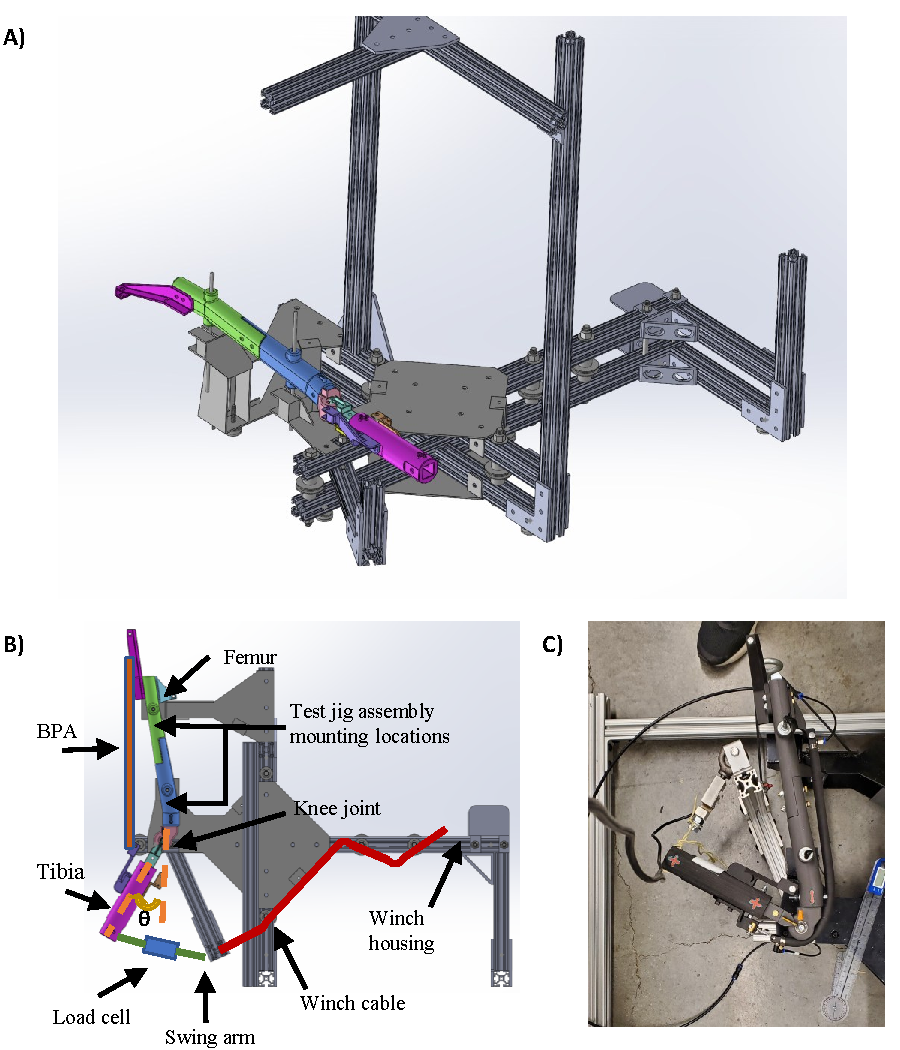
\includegraphics[width=0.73\textwidth]{testJigs_reviewed.pdf}
    \end{center}
    \caption{Pinned-knee test apparatus: CAD assembly (A), labeled mechanism at \ang{-30} (B), and extensor isometric test at \ang{-120} (C).}\label{fig:testJigs}
\end{figure}

The leg assembly geometry and dimensions are based on bones scans of a $6 \, \text{ft}$  (\qty{1.83}{\metre}) tall person \citep{bolen_determination_2019,seth_opensim_2018,delp_interactive_1990,delp_opensim_2007}. Two knee joints were tested, one pure rotational joint, and one biomimetic joint with rotation and translation. Each joint is driven by two antagonistic Festo actuators. Both robot joints have the same center of rotation in the femur frame at $\theta_{\mathbf{k}}=0 \deg$.

Details on the biomimetic robot knee used in this study can be found in \citep{steele_biomimetic_2018,steele_development_2017,steele_biomimetic_2018-1}. In brief, this 1-DoF joint (Figure~\ref{fig:ICR}) uses a four-bar linkage to change the effective moment arm during rotation. The intersection point of the internal crossed links define the instantaneous center of rotation (ICR). This causes the joint ICR location in the femur frame to translate posteriorly in the $X$ direction and distally in the $Y$ direction except for a brief proximal move near full flexion. Reference International Society of Biomechanics (ISB) coordinate frames are given by \citet{wu_for_1995,wu_isb_2002}. This is similar to how the human knee behaves \citep{bolen_determination_2019,morrow_optimization_2020,seth_opensim_2018,delp_opensim_2007,delp_interactive_1990}. The correct location of the ICR is important for both theoretical and experimental torque calculations.



\begin{figure}[htbp]
    \begin{center}
    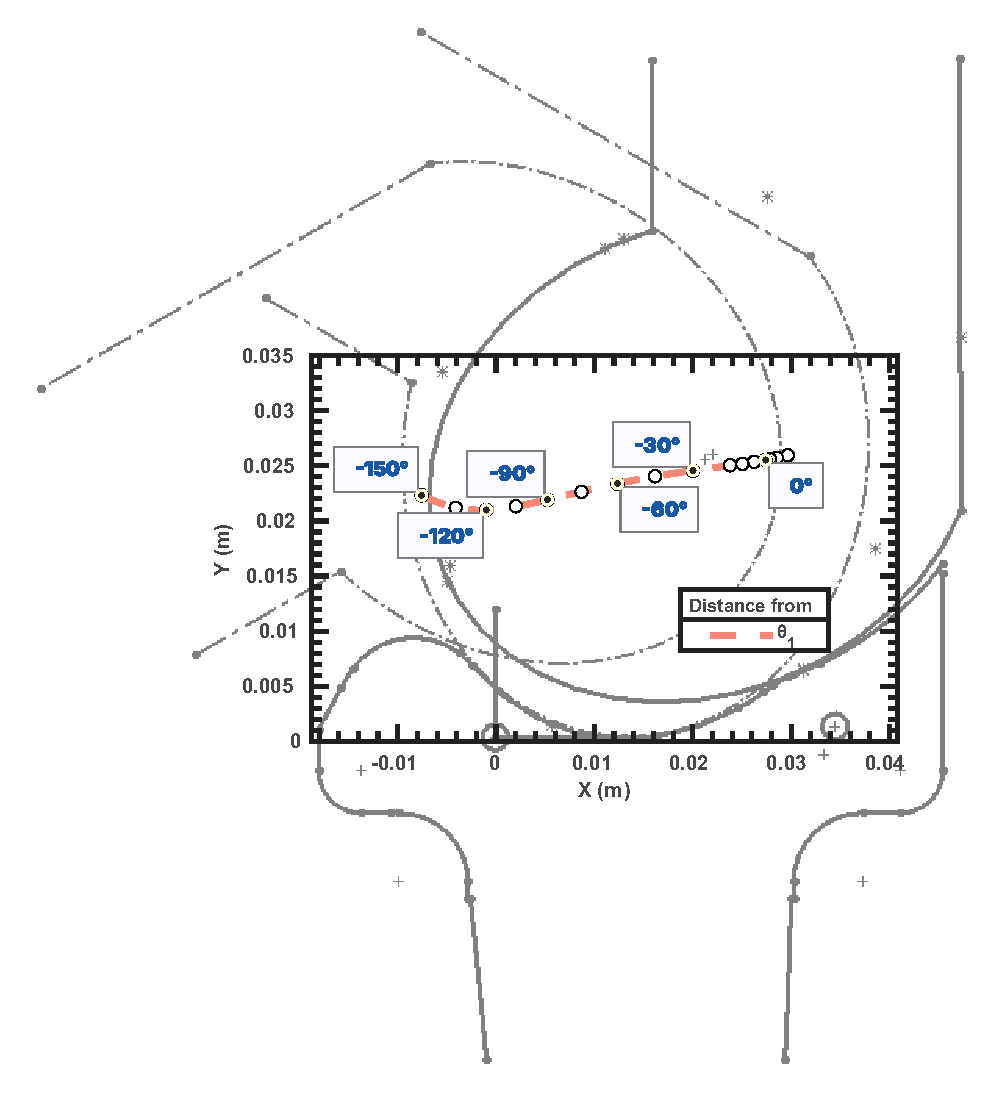
\includegraphics[width=0.8\textwidth]{KneeICR.eps}
    \end{center}
    \caption{Biomimetic-knee instantaneous center of rotation relative to the tibial frame. White circles are measured points; knee outlines show \ang{0} (solid), \ang{-60}, and \ang{-120} (dash-dot).}\label{fig:ICR}
\end{figure}

Both knee types use uniarticular flexor and extensor actuators. Each knee joint type was tested with a single $\diameter$\qty{10}{\mm} Festo BPA per muscle. The biomimetic knee was additionally tested with $\diameter$\qty{20}{\mm} Festo BPAs in a paired configuration: the extensor with two BPAs in parallel, and the flexor with two BPAs whose pathways are mirrored about the $Z$ axis. Each artificial muscle is pinned at the muscle origin location on the femur while the other end is either pinned or attached to the muscle insertion location on the tibia via an artificial tendon.

The modeled geometry and torque calculation follow \citet{bolen_determination_2019,morrow_optimization_2020}. Torque about the knee is generated by the moment of the BPA force about the joint's instantaneous center of rotation (ICR). Two vectors enter that moment: the position vector $\mathbf{d}$, drawn from the ICR to the point where the actuator force is applied, and the force vector $\mathbf{F} = \norm{\mathbf{F}}\hat{\mathbf{u}}$, whose direction $\hat{\mathbf{u}}$ is the line of action of the actuator. The moment of the force about the joint is $\mathbf{M} = \mathbf{d} \times \mathbf{F}$, and the signed knee-axis torque is $M_{\mathbf{k}}=\hat{\mathbf{z}}_{\mathbf{k}}\cdot(\mathbf{d}\times\mathbf{F})$. For force acting in the plane normal to the knee axis, the moment-arm magnitude is

\begin{equation}
    r = \norm{\mathbf{d} \times \hat{\mathbf{u}}}
    \label{eq:momentarm_def}
\end{equation}

This planar moment arm is a scalar distance and can be computed from the vectors or measured directly. For an out-of-plane force, the knee-axis moment must instead use the axis projection above; the magnitude of the full three-dimensional moment is not generally the knee torque. In this study it is calculated using the method specified by \citet{young_analyzing_2019}. The scalar moment arm $r_{\mathbf{k}}$ about the joint axis $\hat{\mathbf{z}}_{\mathbf{k}}$ (i.e., the $Z$ axis in the knee frame) is calculated as 

\begin{equation}
    r_{\mathbf{k}} = \mathbf{p}_{proj,xy} \cdot \frac{\mathbf{p}_{f} \times \hat{\mathbf{z}}_{\mathbf{k}}} { \norm{\mathbf{p}_{f} \times \hat{\mathbf{z}}_{\mathbf{k}}} } \label{eq:project_ma}
\end{equation}

A muscle path may be modeled as a single segment running from origin to insertion, or as a chain of segments joined at via points. The segment that crosses from one reference frame into the other, here from the femur frame to the tibia frame, is the free muscle segment: because its endpoints ride on different bodies, its length and its direction respond directly to joint rotation, whereas a segment contained within one body's frame rotates rigidly with that body and changes neither. Here $\mathbf{p}_{f}$ is the force-path segment vector, and $\mathbf{p}_{proj,xy}$ locates a point on that line relative to the joint, projected onto the plane normal to the joint axis. The normalized cross product in Equation~\eqref{eq:project_ma} is the in-plane normal to the force path. Its dot product with the projected position gives the signed moment arm of the projected force path (Figure~\ref{fig:masters_routing_and_arms}). Multiplying this arm by the in-plane force magnitude gives the knee-axis torque; the full wrench calculation retains all three force components. Moment arm is calculated in the tibial body frame.



\subsection{Knee Torque Data Collection and Equipment}\label{sec:torque_equipment}


A test jig was built to collect knee torque measurements at different knee angles over its range of motion. The test stand frame is made predominantly out of 80/20 1515 series extruded aluminum components. The knee joint is free to rotate the tibia while the femur is fixed to the frame. A force sensor has one end connected to the tibia and the other is connected to a swing arm. The swing arm is tied to a winch with $3/16\; \text{inch}$ Kevlar rope from Quality Nylon Rope routed over intermediate idler pulleys (see Figure~\ref{fig:testJigs}\textbf{(B)} and Figure~\ref{fig:testJigs}\textbf{(C)}). At each measured position of $\theta_{\mathbf{k}}$ the winch would be locked and the BPA would be inflated and then deflated. This test procedure kept the measured results as isometric as possible.  The knee joint is co-axial with gravity to eliminate gravitational torque (see Figure~\ref{fig:testJigs}\textbf{(A)} and Figure~\ref{fig:testJigs}\textbf{(C)}).

Force data was collected using one of two different sensors. The first is a MODERN STEP $\qty{300}{\kilo\gram}$ digital crane scale. The second force sensor is a CALT DYLY-103 $\qty{100}{\kilo\gram}$ S shaped load cell. The load cell is used in conjunction with a HX711 Load Cell Amplifier. Pressure is measured with a Freescale MPX5700 GP $\qty{5}{\volt}$ pressure sensor. Building air supply pressure is controlled with two pressure regulators in series. The first is a Parker model 20R113GC $0-120\; \text{psi}$ pressure regulator. The second is a Husky $3/8 \; \text{inch}$ High Performance Air Regulator HDA72200. A Festo VTUG-10-MRCR-S1T-26V20-T516LA-UL-T532S-8K valve manifold was used to supply air to the actuator. Pressure and load cell amplifier data are sent to MATLAB via an Arduino Uno style Sparkfun BlackBoard C microcontroller. 


The length measurements were made using a tape measure. When there was sufficient curvature in the BPA during knee extensor torque tests, a flexible piece of string was used to mark the axial length and then transferred to the tape measure. Angle measurements were taken with a Medigauge digital electronic goniometer or with MALENOO analog goniometers of 6, 8, or 12 inch lengths.  

\subsection{Hybrid Torque Calculation Method}\label{sec:hybrid_method}


The hybrid torque calculation measures the actual muscle length and angles of the robot to calculate force and joint torque, isolating which part of the torque equation did not achieve its predicted value. The classical mechanics way to calculate the torque about a joint is to take the cross product of the position vector $\mathbf{d}$ and the force vector $\mathbf{F}$, both defined in Section~\ref{sec:robot_model},

\begin{equation}
    \mathbf{M} = \mathbf{d} \times \mathbf{F} \label{eq:M_vec}
\end{equation}

Knee torque is the scalar component of this moment about the joint axis, written $M_{\mathbf{k}}$ to make its axis explicit. For the planar hybrid calculation, its magnitude is the measured perpendicular arm multiplied by the actuator-force magnitude,

\begin{equation}
    \abs{M_{\mathbf{k}}} = r\,F \label{eq:M_scalar}
\end{equation}

where $r$ is the scalar moment arm of Eq.~\eqref{eq:momentarm_def}, here measured directly with a tape measure as the perpendicular distance from the knee axis to the actuator's line of action, and $F$ is the scalar force magnitude, calculated by measuring the BPA's $P$, $l_{0}$, $l_{620}$ and $l_\text{m}$ values and using the model fit equations determined in the previous chapter. The hybrid method therefore replaces the model-predicted moment arm $r_{\mathbf{k}}$ of Eq.~\eqref{eq:project_ma} and the model-predicted muscle length with their measured counterparts, leaving the force model as the only predicted quantity. The flexor and extensor signs are then assigned using the adopted knee convention.

\subsection{Improved Torque Model}\label{sec:improved_model}

The classical torque calculation treated links and attachments as rigid: the routed path depended on joint geometry but did not change under actuator load. Data collected during the first flexor experiments (Section~\ref{sec:results_torque}) showed that this assumption does not hold for a pneumatic system: measured muscle lengths were consistently shorter than predicted, and measured torque deviated from prediction in a load-dependent manner. This section describes the corrections that were developed to account for a constant length offset, series compliance in the attachment hardware and artificial tendons, and the loss of usable muscle length when a BPA wraps around the joint.

The correction terms represent the combined effects of the attachment brackets, fixtures, artificial tendons, and test-stand loading path. They are identified from measured torque because the torque prediction requires their aggregate effect on actuator length, rather than a separate structural model of every component. The constant term $\chi_0$ corrects the unloaded length discrepancy, $\chi_1$ and $\chi_2$ describe effective stiffness in the local bracket frame, and $\chi_3$ scales the wrapping-length loss. The compliance calculation couples force and displacement: force deflects the attachments, and the resulting change in muscle length changes force. The multiobjective procedure of Section~\ref{sec:identification} evaluates candidate terms on fitting and validation tests.

\subsubsection{Length Offset and System Stiffness}\label{sec:offset_stiffness}

Measured muscle length was consistently shorter than predicted at all joint angles, producing less muscle force, a shifted RoM, and less torque in the experimental setup. Because the discrepancy persists at $\varepsilon=1$ and $F=0$, where no compliance can act, the correction is a constant length offset: $l_\text{m}$ was recalculated as

\begin{equation}
    l_\text{m} = l_{LMT} - 2\;l_{fitting} - \chi_{0} 
    \label{eq:Lm}
\end{equation}

where $l_{LMT}$ is the path length of the musculotendon from origin to insertion point, $l_{fitting}$ is the length of the end caps, and $\chi_{0}$ is a constant length offset. 

Actuator force deforms the attachments, changing effective BPA length and the predicted force. I approximate this load-dependent deformation with Hooke's law along the bracket-frame principal directions. The fitted stiffnesses $\chi_1$ and $\chi_2$ represent the combined attachment system, not direct measurements of individual hardware components. Because fixtures and loading hardware contribute to that compliance, beam theory alone cannot determine the fitted values.

A local bracket frame was established at the attachment bracket. The $\hat{\mathbf{x}}_{br}$ axis was aligned with the vector from the bracket reference point to the BPA attachment point and represents the stiffest direction of the bracket. The $\hat{\mathbf{y}}_{br}$ axis was chosen to point in the posterior direction with respect to the tibia frame, corresponding to the primary cantilever bending direction (see Figure~\ref{fig:bktFrame}), while the $\hat{\mathbf{z}}_{br}$ axis completes the right-handed frame. In this frame the bracket is modeled as three independent linear springs along the principal axes, with stiffnesses $k_{x}$, $k_{y}$, and $k_{z}$ in the $x_{br}$, $y_{br}$, and $z_{br}$ directions.

\begin{figure}[htbp]
\begin{center}
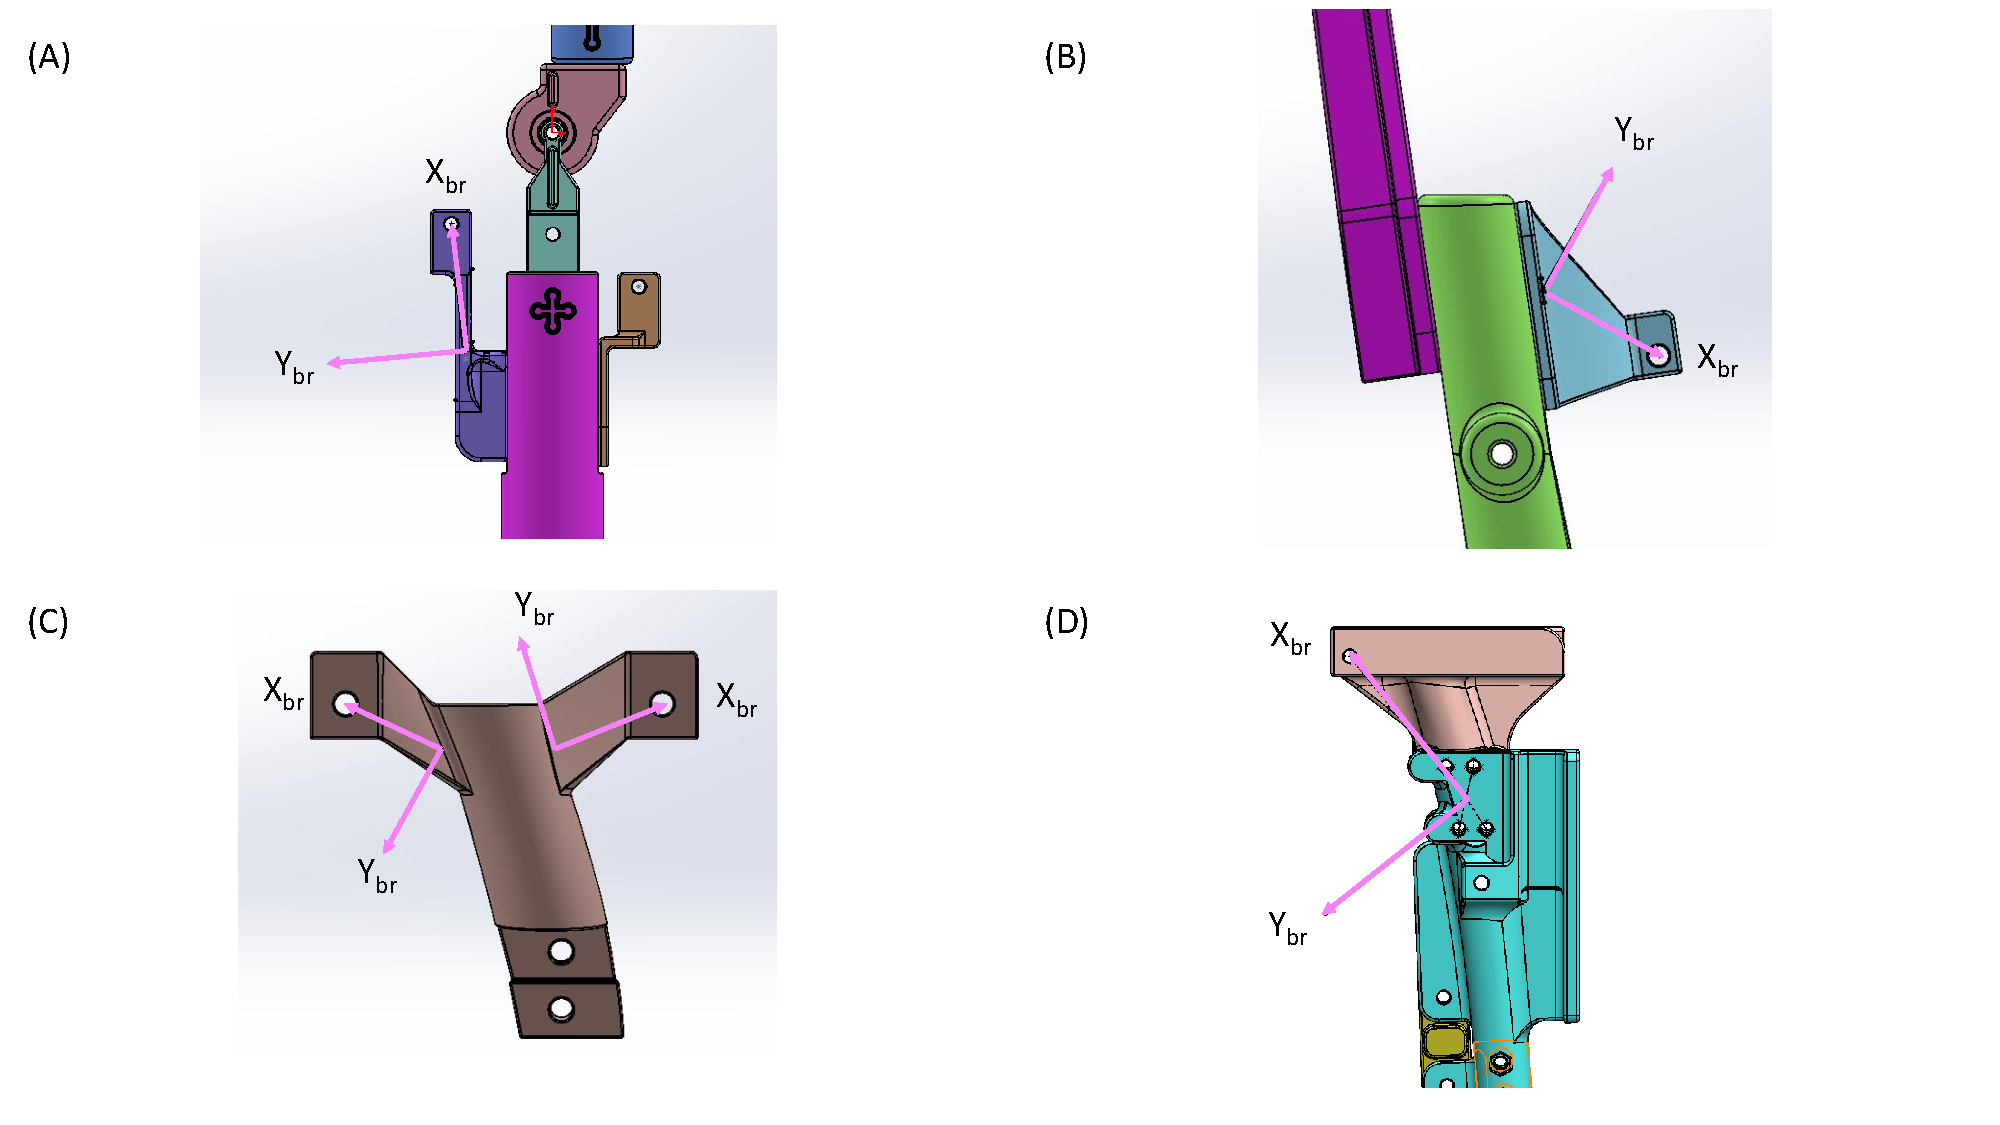
\includegraphics[width=1\textwidth]{bktFrame.pdf}
\end{center}
\caption{Bracket frame orientations for: \textbf{(A)} flexor configuration on the pinned knee, \textbf{(B)} extensor configuration on the pinned knee, \textbf{(C)} flexor and extensor configurations on the biomimetic knee with $\diameter$\qty{10}{\mm} BPAs, and \textbf{(D)} flexor configuration on the biomimetic knee with the $\diameter$\qty{20}{\mm} BPA.}
\label{fig:bktFrame}
\end{figure}

Both attachment brackets, the insertion-side bracket on the tibia and the origin-side bracket on the femur, carry two-rotation frames: a yaw $\theta_z$ about the fixed space-frame axis $\hat{\mathbf{z}}_{s}$ followed by a pitch about the current $\hat{\mathbf{y}}_{br}$ axis aligns $\hat{\mathbf{x}}_{br}$ with the vector from the bracket origin to its attachment point, $\mathbf{p}_{B}$ on the insertion bracket and $\mathbf{p}_{A}$ on the origin bracket (Figure~\ref{fig:xiFrameTransform}). Appendix~\ref{app:model_geometry} records both frames, their reference points, and their stiffness forms (Equation~\eqref{eq:app_bracketframe}, Tables~\ref{tab:app_bracket_points} and~\ref{tab:app_stiffness_arrays}). The resulting orientation and homogeneous transform are

\begin{equation}
\mathbf{R}_{sb}=\mathbf{R}_z(\theta_z)\mathbf{R}_y(\theta_y)^T.
\label{eq:bracket_frame_rotation}
\end{equation}
\begin{equation}
\mathbf{T}_{sb}=
\begin{bmatrix}
\mathbf{R}_{sb} & \mathbf{p}_{br}\\
\mathbf{0}^{T} & 1
\end{bmatrix}.
\label{eq:bracket_frame_transform}
\end{equation}

\begin{figure}[htbp]
\centering
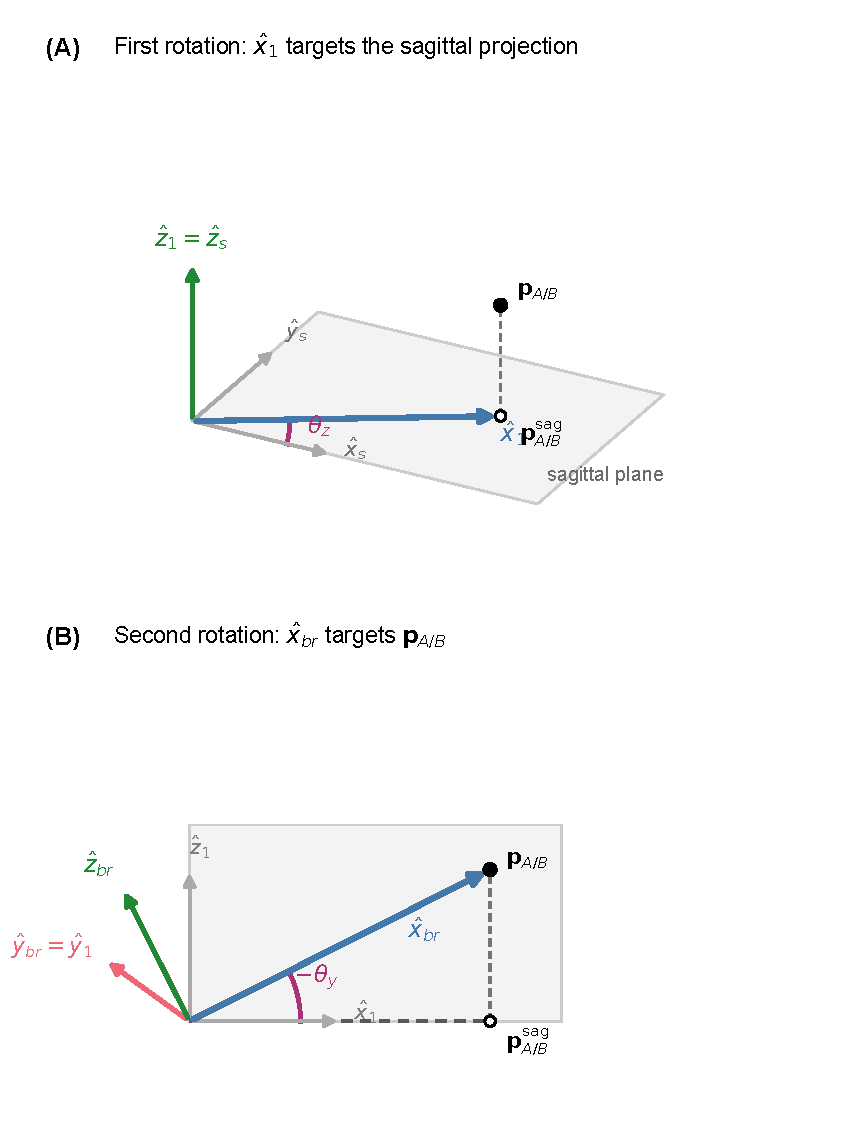
\includegraphics[height=0.72\textheight]{xiFrameTransform.pdf}
\caption{Bracket-frame construction from attachment point $\mathbf{p}_A$ or $\mathbf{p}_B$: yaw about fixed $\hat{\mathbf z}_s$ aligns the sagittal projection (A); pitch about current $\hat{\mathbf y}_{br}$ aligns the full point vector (B).}
\label{fig:xiFrameTransform}
\end{figure}



\begin{equation}
\mathbf{K}_{br} = \operatorname{diag}\!\left(k_{x},\; k_{y},\; k_{z}\right)
\label{eq:bktstiffness_general}
\end{equation}

The fitted values $\chi_1$ and $\chi_2$ define the principal stiffnesses, with configuration-specific axis assignments in Table~\ref{tab:app_stiffness_arrays}. The adopted pinned-flexor fit uses two brackets with two-rotation frames. For the insertion bracket, $k_x=k_z=\chi_1$ and $k_y=\chi_2$; this symmetric assignment makes rotation about $\hat{\mathbf y}_{br}$ immaterial to its compliance. The origin bracket uses $[\chi_1,\chi_1,\chi_2]$, for which that invariance does not hold. Appendix~\ref{app:model_geometry} records the remaining assignments. For the insertion bracket,

\begin{equation}
\mathbf{K}_{br} = 
\begin{bmatrix}
\chi_{1} & 0   & 0 \\
0   & \chi_{2} & 0 \\
0   & 0   & \chi_{1} \\
\end{bmatrix}
\label{eq:bktstiffness}
\end{equation}

The corresponding local compliance matrix is 

\begin{equation}
\mathbf{C}_{br} = \mathbf{K}_{br}^{-1}
\label{eq:bktcompliance}
\end{equation}

The force applied to the bracket was expressed in the bracket frame as $\mathbf{F}_{br}$. This force vector can be written in terms of its magnitude and unit direction as

\begin{equation}
\mathbf{F}_{br} = F \, \hat{\mathbf{u}}
\label{eq:bktforcevector}
\end{equation}
\noindent
where $F = \norm{\mathbf{F}}$ is the scalar force magnitude of Eq.~\eqref{eq:M_scalar} and $\hat{\mathbf{u}} = [u_{x}, u_{y}, u_{z}]^{T}$ is the BPA force direction expressed in the bracket frame. The bracket deflection vector, $\boldsymbol{\epsilon}_{br}$, was calculated from Hooke's law as 

\begin{equation} \mathbf{F}_{br} = \mathbf{K}_{br} \: \boldsymbol{\epsilon}_{br}
\label{eq:bktvectorhooke}
\end{equation}

Solving Eq. \ref{eq:bktvectorhooke} for the bracket deflection gives

\begin{equation}
\boldsymbol{\epsilon}_{br} = \mathbf{K}_{br}^{-1} \: \mathbf{F}_{br} = \mathbf{C}_{br} \: \mathbf{F}_{br}
\label{eq:bktdeflection}
\end{equation}

Substituting Eq. \ref{eq:bktforcevector} into Eq. \ref{eq:bktdeflection} gives

\begin{equation}
\boldsymbol{\epsilon}_{br} = F \,\mathbf{K}_{br}^{-1} \,\hat{\mathbf{u}}
\label{eq:bktdeflectionforceunit}
\end{equation}

For the diagonal stiffness matrix in Eq. \ref{eq:bktstiffness}, Eq. \ref{eq:bktdeflection} is equivalent to the component-wise expression

\begin{equation}
\boldsymbol{\epsilon}_{br} = \begin{bmatrix} F\,u_{x}/\chi_{1} \\ F\,u_{y}/\chi_{2} \\ F\,u_{z}/\chi_{1} \end{bmatrix}
\label{eq:bktcomponentdeflection}
\end{equation}

Only the component of the three-dimensional deflection vector $\boldsymbol{\epsilon}_{br}$ along the BPA line of action changes the effective BPA length, so the scalar bracket deflection entering the force model is its projection onto $\hat{\mathbf{u}}$:

\begin{equation}
{\delta}_{br} = \hat{\mathbf{u}}^{T} \boldsymbol{\epsilon}_{br}
\label{eq:bktprojecteddeflection}
\end{equation}

Substituting Eq. \ref{eq:bktdeflection} into Eq. \ref{eq:bktprojecteddeflection} gives

\begin{equation}
{\delta}_{br} = \hat{\mathbf{u}}^{T} \, \mathbf{K}_{br}^{-1} \, \mathbf{F}_{br}
\label{eq:bktprojecteddeflection2}
\end{equation}

Using Eq. \ref{eq:bktforcevector}, Eq. \ref{eq:bktprojecteddeflection2} becomes

\begin{equation}
\delta_{br} = F\, \hat{\mathbf{u}}^{T} \, \mathbf{K}_{br}^{-1} \, \hat{\mathbf{u}}
\label{eq:bktprojectedcompliance}
\end{equation}

With $\mathbf{C}_{br}=\mathbf{K}_{br}^{-1}$, the scalar compliance along the BPA line of action is

\begin{equation}
c_{\hat{u},br} = \frac{\delta_{br}}{F} = \hat{\mathbf{u}}^{T} \mathbf{C}_{br} \hat{\mathbf{u}}
\label{eq:keff}
\end{equation}

This projected-compliance form is used because the force is applied along $\hat{\mathbf{u}}$, while the bracket is allowed to deflect independently along its local $\hat{\mathbf{x}}_{br}$, $\hat{\mathbf{y}}_{br}$, and $\hat{\mathbf{z}}_{br}$ directions. The reduced-order Hooke's law expression for the bracket deflection along the BPA line of action is therefore

\begin{equation} F = k_{eq} \: \delta
\label{eq:hookereduced}
\end{equation}

Here $k_{eq}$ is the equivalent stiffness of every compliant element in the actuator path; with no tendon it reduces to $k_{eq}=c_{\hat{u},br}^{-1}$ of Equation~\eqref{eq:keff}. An artificial tendon is modeled as an axial spring with stiffness $k_{ten}$: bracket deflection and tendon stretch both shorten the effective BPA length along the actuator line of action, the two elements carry the same force, and their scalar compliances add in series.

The projected bracket compliance is $c_{\hat{u},br}=k_{\hat{u},br}^{-1}$, tendon compliance is $c_{ten}=k_{ten}^{-1}$, and the equivalent stiffness is $k_{eq}=c_{eq}^{-1}$.\par
\begin{equation} c_{eq} = c_{\hat{u},br} + c_{ten}
\label{eq:equivalentstiffness}
\end{equation}

The series model assumes quasi-static tensile loading, linear compliance, additive axial displacements, and a tendon without preload. Rotational compliance and force--moment coupling are neglected. Within each force-balance calculation the line of action is fixed; the attachment positions, force direction, and moment arm are then recalculated at the deflected geometry. Antagonistic loading that lengthens the actuator lies outside this treatment.

Since $\delta$ is the scalar compliance displacement along the BPA line of action, then the compliance-corrected active BPA length used in the force balance is

\begin{equation} l_m(\delta) = l_m{(0)} - \delta
\label{eq:activelengthcorrected}
\end{equation}

where $l_m{(0)}$ is the initial muscle length calculated from \eqref{eq:Lm}.

For a specified set of correction parameters, the following calculation solves the attachment-compliance displacement at each knee angle; it is distinct from the optimization that identifies those parameters from experimental torque data (Section~\ref{sec:identification}). The corresponding relative contraction is $\varepsilon^*(\delta)$. Since the BPA force depends on contraction, and contraction depends on the compliance displacement, $\delta$ is the root of the nonlinear force-balance equation

\begin{equation} F_{\mathrm{max}} \cdot F_{\mathrm{BPA}}\!\left(\varepsilon^*(\delta),P^*\right) - k_{eq}\,\delta = 0
\label{eq:complianceforcebalance}
\end{equation}

MATLAB \texttt{fzero} solves Equation~\eqref{eq:complianceforcebalance} between zero displacement and the maximum usable contraction, using its default tolerance. If the actuator is already at that contraction limit or the residual has no sign change, the evaluator returns $\delta=0$. Solver tolerance is distinct from physical-model accuracy.

After solving Equation~\eqref{eq:complianceforcebalance}, I used the force to calculate vector bracket displacement, transformed the displaced attachment into the limb frame, and recalculated routed length, force direction, moment arm, and torque.

The actuator path can carry compliant hardware at both ends: the insertion-side bracket of the preceding development together with a second, origin-side bracket. Figure~\ref{fig:xiProjection} distinguishes the three-dimensional displacement of each bracket from the scalar displacement along the BPA force path. For bracket $j$, the displacement resolves into components $\eta_{1,j}$, $\eta_{2,j}$, and $\eta_{3,j}$ along the local bracket-frame basis, whereas only its projection $\delta_{br,j}$ along the corresponding force direction $\hat{\mathbf{u}}_j$ changes the actuator length. The two bracket projections act in series with the tendon elongation $\delta_{\mathrm{tendon}}$:

\begin{equation}
\begin{aligned}
\boldsymbol{\eta}_{br,j} &= \sum_{i=1}^{3}\eta_{i,j}\hat{\mathbf{e}}_i^{(j)},\\
\delta_{br,j} &= \hat{\mathbf{u}}_j^T\boldsymbol{\eta}_{br,j}, \qquad j\in\{1,2\},\\
\delta_{\mathrm{series}} &= \delta_{br,1}+\delta_{\mathrm{tendon}}+\delta_{br,2}.
\end{aligned}
\label{eq:bracket_series_projection}
\end{equation}

\begin{figure}[htbp]
\centering
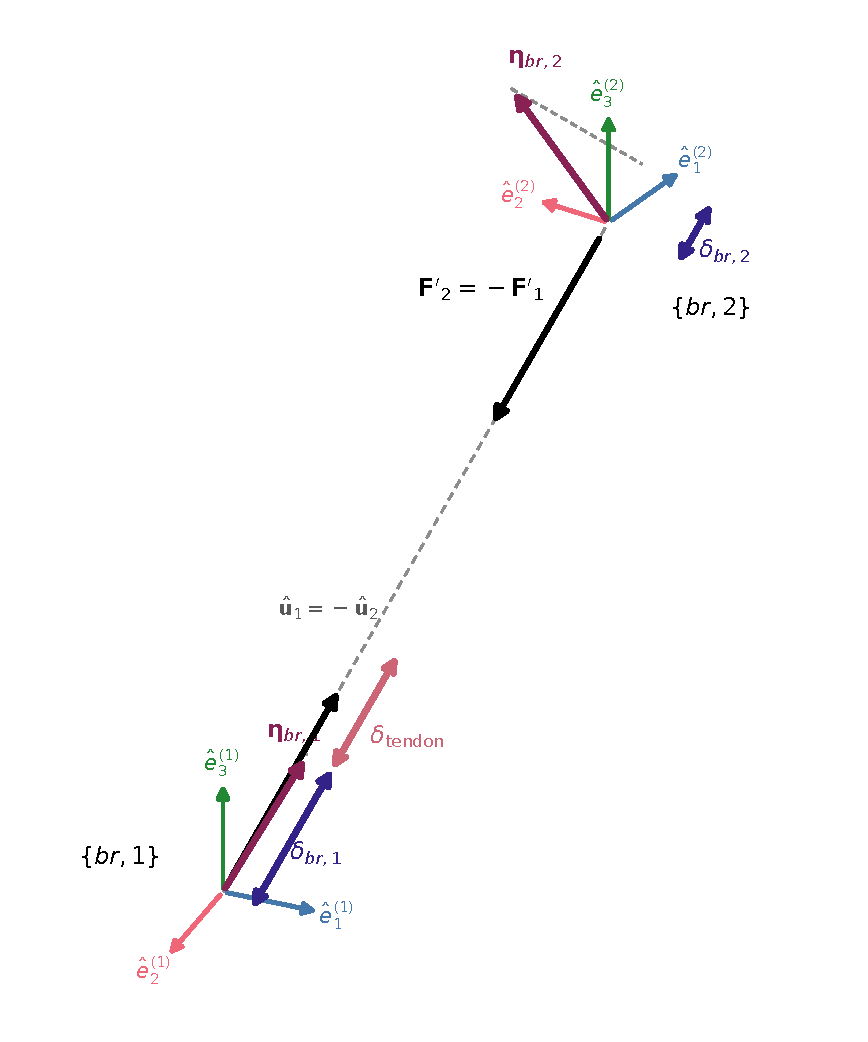
\includegraphics[width=0.72\textwidth,height=0.62\textheight,keepaspectratio]{xiProjection.pdf}
\caption{Projection of bracket displacement onto the actuator force path. Each bracket has a local basis $\hat{\mathbf e}^{(j)}_1$, $\hat{\mathbf e}^{(j)}_2$, and $\hat{\mathbf e}^{(j)}_3$. The displacement $\boldsymbol\eta_{br,j}$ has an axial projection $\delta_{br,j}$ along $\hat{\mathbf u}_j$; the two bracket projections and tendon elongation contribute to the change in actuator length. Displacements are exaggerated.}
\label{fig:xiProjection}
\end{figure}


\subsubsection{BPA Fictive Contraction}\label{sec:fictive_contraction}

As the knee flexes, the extensor BPA contacts the anterior joint surface and bends around it (Figure~\ref{fig:bpaWrapping}). The rigid routed-length calculation does not account for the resulting change in usable contraction. I represent this effect with fictive strain: an empirical increase in the contraction seen by the force model, beyond the actuator's geometric contraction. The correction is phenomenological; it does not resolve wall stresses or the deformation of the braided actuator. A wrapping-loss term $\chi_3$ scales the associated reduction in usable length:
\begin{equation}
    \Delta l = \begin{cases}
     \chi_{3}\;R\;\abs{ \theta_{\mathrm{wrap}}-\theta_{\mathbf{k}}}\;\zeta^2 & \theta_{\mathbf{k}} \leq      \theta_{\mathrm{wrap}} \\
      0 & \theta_{\mathbf{k}} \geq \theta_{\mathrm{wrap}}
     \end{cases}\label{eq:deltaL}
\end{equation}

where $\Delta l$ is the change in usable length of the BPA, $R$ is the wrapping radius, $\abs{\theta_{\mathrm{wrap}}-\theta_{\mathbf{k}}}$ is the angle through which the BPA is bent once contact begins, and $\theta_{\mathrm{wrap}}$ is the knee flexion angle at which the BPA starts to bend over the knee joint, determined from solid modeling. $\zeta$ is the additive complement to relative strain, such that

\begin{equation}
    \zeta = 1-\varepsilon^*  \\
\label{eq:comp}
\end{equation}

so the fitted wrapping loss grows quadratically toward resting length and vanishes at the normalized free-contraction limit. Combining \eqref{eq:comp} into \eqref{eq:deltaL}, and subtracting $\Delta l$ from  \eqref{eq:Lm} yields

\begin{equation}
    l_\text{m} = l_{LMT} - 2\;l_{fitting}  - \chi_{0} - \Delta l\label{eq:x3}
\end{equation}

Figure~\ref{fig:bpaWrapping} shows a sagittal schematic of an extensor BPA crossing a flexed robot knee, with its braided body following an anterior contact arc between the proximal attachment and distal tendon. Dashed radii bound the contact arc; $R$ is the BPA-path wrapping radius, and $\alpha=\abs{\theta_{\mathrm{wrap}}-\theta_{\mathbf{k}}}$ is the bend angle after contact begins, expressed in radians in Equation~\eqref{eq:deltaL}. The drawing illustrates the local circular-wrap approximation, not the full multi-contact route. The fitted usable-length loss $\Delta l$ is not an arc-minus-chord length.

\begin{figure}[htbp]
\centering
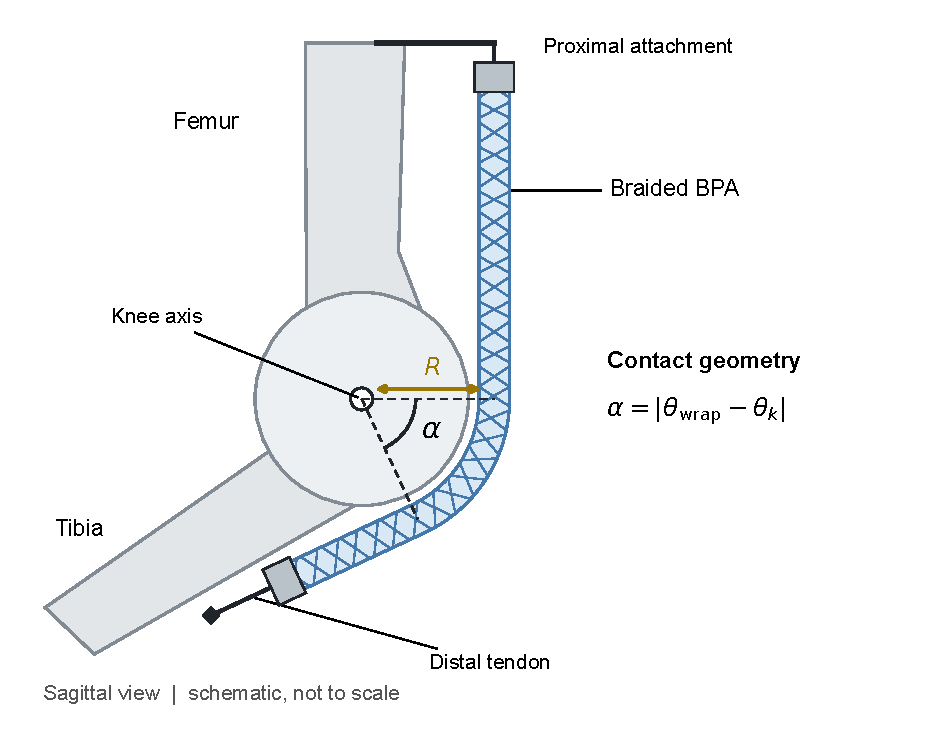
\includegraphics[width=\textwidth]{bpa_knee_wrapping_review.pdf}
\caption[BPA crossing a flexed knee]{Extensor BPA wrapping around a flexed knee. Dashed radii bound the local contact arc, with wrapping radius $R$ and bend angle $\alpha$.}
\label{fig:bpaWrapping}
\end{figure}

\subsubsection{Identification of the Torque-Model Correction Terms}\label{sec:identification}

I set the correction terms in two stages using \texttt{gamultiobj} in MATLAB. The flexor stage fits $(\chi_0,\chi_1,\chi_2)$ with compliance at both attachments. The selected training/validation split trains on the $l_0=\qty{48.5}{\cm}$ and \qty{41.0}{\cm} tests and validates on the \qty{45.7}{\cm} and \qty{40.6}{\cm} tendon tests. The extensor stage locks $(\chi_1,\chi_2)$ to that same flexor-front member and fits only $(\chi_0,\chi_3)$. Its selected training/validation split trains on the \qty{43.6}{\cm}, \qty{43.2}{\cm}-tendon, and \qty{45.7}{\cm} tests and validates on the \qty{40.0}{\cm} plain, \qty{40.0}{\cm}-tendon, and \qty{46.5}{\cm} tests. The extensor length offset is allowed to be negative. Appendix~\ref{app:model_geometry} records the test constants, bounds, stiffness-axis assignments, and adopted values in Tables~\ref{tab:app_flxpin_tests}, \ref{tab:app_extpin_tests}, \ref{tab:app_opt_bounds}, \ref{tab:app_stiffness_arrays}, and~\ref{tab:AdoptedXi}.



Each candidate is evaluated using RMSE, FVU, and maximum absolute residual. These metrics jointly measure torque error; none isolates a unique source such as level offset, waveform shape, or angular misalignment.

The objective vector of the identification is defined explicitly. For a candidate correction vector $\boldsymbol{\chi}$, $(\chi_{0}, \chi_{1}, \chi_{2})$ in the flexor stage and $(\chi_{0}, \chi_{3})$ on the locked stiffness pair in the extensor refit, the predicted torque curve of test $i$ is interpolated to its $n_{i}$ measured knee angles $\theta_{ij}$, giving residuals $e_{ij} = M_{ij} - \hat{M}(\theta_{ij}; \boldsymbol{\chi})$ against the measured torque $M_{ij}$, and the three goodness-of-fit components of that test are
\begin{equation}
\mathrm{RMSE}_{i} = \sqrt{\frac{1}{n_{i}}\sum_{j} e_{ij}^{2}}\label{eq:gof_components}
\end{equation}
\begin{equation}
\mathrm{FVU}_{i} = \frac{n_{i}-1}{n_{i}} \cdot \frac{\sum_{j} e_{ij}^{2}}{\sum_{j} (M_{ij} - \bar{M}_{i})^{2}}\label{eq:gof_fvu}
\end{equation}
\begin{equation}
e^{\max}_{i} = \max_{j} \abs{e_{ij}}.\label{eq:gof_max}
\end{equation}
FVU expresses the residual sum of squares relative to the sum of squared deviations of the measured torque from its mean $\bar{M}_{i}$, with the factor $(n_{i}-1)/n_{i}$ carrying the small-sample adjustment of the evaluators; RMSE and the maximum absolute residual carry torque units, whereas FVU is dimensionless. For a given test, FVU is proportional to squared RMSE, so the two metrics are not independent measures of shape and level, and across tests their different scaling changes the relative weighting of the errors. The solver minimizes the objective vector
\begin{equation}
\mathbf{g}(\boldsymbol{\chi}) = \frac{1}{\abs{\mathcal{T}}} \sum_{i \in \mathcal{T}}
\begin{bmatrix}
g_{1,i}(\boldsymbol{\chi})/g_{1,i}^{(0)} \\
g_{2,i}(\boldsymbol{\chi})/g_{2,i}^{(0)} \\
g_{3,i}(\boldsymbol{\chi})/g_{3,i}^{(0)}
\end{bmatrix},
\label{eq:gof_objective}
\end{equation}
where $g_{1,i}$, $g_{2,i}$, and $g_{3,i}$ are the RMSE, FVU, and maximum absolute residual of Equations~\eqref{eq:gof_components}--\eqref{eq:gof_max}, the superscript $(0)$ marks the zero-correction baseline value of the same component, the same kinematics and force model with every correction term disabled, and $\mathcal{T}$ is the set of tests used for training. The mean of the baseline-normalized components makes the three objectives dimensionless and the training tests commensurate. The search carried no constraints beyond the parameter bounds of each stage, and the returned Pareto fronts (the candidate parameter sets for which improving one objective requires worsening another) were filtered to members scoring at or below the zero-correction baseline on every component of every test in that stage's identification pool.

MATLAB \texttt{gamultiobj} uses NSGA-II to return the Pareto front \citep{deb_nsga2_2002, mathworks_optimization_2025}. Candidate predictions are checked on the training and validation tests. The search uses bounded, normalized parameters, with logarithmic stiffness coordinates. Population, mutation, crossover, and stopping settings are retained with the archived run records.

\subsection{Actuator Placement and Route Redesign}\label{sec:mesh_opt}\label{sec:optimization}

The placement search varies actuator attachments to control moment arm and muscle excursion over the joint range of motion \citep{bolen_determination_2019,morrow_optimization_2020}. For the erector spinae, internal oblique, and external oblique at the lumbosacral joint, the targets are Gait2392 torque surfaces sampled at 100 positions along each of two joint coordinates.

At each scale the search perturbs both attachments by $\pm\epsilon$ offsets along the Cartesian coordinates (eight candidates per attachment, 64 candidate pairs), centers on the lowest-cost pair, and halves $\epsilon$ when no candidate improves, from an initial $\epsilon=\qty{0.1}{\m}$ down to \qty{1}{\mm} \citep{morrow_optimization_2020}.

The original cost combined the summed absolute torque mismatch over the sampled poses, actuator length, displacement of the attachments from their starting locations, and a diameter-dependent penalty. The published weights for the first three terms were $10^{-4}$, $10^{-2}$, and $1$, respectively; the penalties for \qtylist{10;20;40}{\mm} BPAs were $1$, $5$, and $15$. These were numerical weights chosen to balance differently scaled cost terms. The geometric terms discouraged impractical placements but did not impose collision avoidance: attachments could lie away from the modeled bones, and routes could intersect them. This study established the placement-search approach; it did not establish physical torque accuracy or satisfaction of the human torque requirement at every pose.

A subsequent knee implementation restricted candidates to mesh points on the femur and tibia: for the biceps femoris short-head replacement, every origin--insertion pair was evaluated over 100 knee poses from approximately \ang{-120} to \ang{10} at a fixed \qty{20}{\mm} diameter, candidates outside the allowable contraction range were rejected, and the lowest-cost usable pair was retained. Like the earlier cube-perturbation search, this discrete mesh search used rigid attachment geometry without the experimentally identified compliance corrections.

The knee-flexor mesh search also used a different objective from the original torque-mismatch cost. It rewarded torque surplus in the human torque's direction while penalizing disagreement between the human and robot torque-vector directions:
\begin{equation}
C_{\mathrm{mesh}} = -\frac{1}{3N}\sum_{j=1}^{N}\left[\,w_{\mathbf{k}}\,D_{\mathbf{k},j} + \sum_{a\in\{x,y\}} w_{a}\,D_{a,j}\right] + \frac{w_{u}}{N}\sum_{j=1}^{N}\left(1 - \hat{\mathbf{M}}^{\mathrm{H}}_{j}\cdot\hat{\mathbf{M}}^{\mathrm{R}}_{j}\right).
\label{eq:mesh_reward}
\end{equation}
Here $N$ is the number of evaluated poses, and $D_{a,j}=M^R_{a,j}-M^H_{a,j}$ when $M^H_{a,j}\geq0$, with the subtraction reversed otherwise; Table~\ref{tab:mesh_original_weights} records the weights and their meaning. A zero robot-torque vector is assigned the opposite human direction in the direction term, which assumes a nonzero human torque vector at the evaluated pose. Torques are supplied in newton meters; this is a numerically weighted score, rather than a sum of normalized physical errors, and minimizing it favors torque capacity in the required direction without guaranteeing that the requirement is met at every pose.




\begin{table}[htbp]
\caption{Terms of the knee-flexor mesh-placement cost. The cost is minimized; a surplus reduces it, while a direction mismatch increases it.}
\label{tab:mesh_original_weights}
\begin{tabularx}{\textwidth}{@{}p{0.24\textwidth}p{0.12\textwidth}X@{}}
\toprule
\textbf{Term} & \textbf{Weight} & \textbf{Meaning} \\
\midrule
Knee torque surplus & $5$ & Signed surplus $D_{\mathbf{k},j}$, summed with the off-axis terms and divided by $3N$; enters with a negative sign. \\
Off-axis torque surplus & $0.25$ each & Signed surplus $D_{x,j}$ and $D_{y,j}$, using the human torque's sign on each axis; enters with a negative sign. \\
Direction mismatch & $10$ & Mean $1-\hat{\mathbf{M}}^H_j\cdot\hat{\mathbf{M}}^R_j$; zero for aligned vectors and two for opposing vectors. \\
\bottomrule
\end{tabularx}
\end{table}

\subsection{Constrained Knee-Route Redesign}\label{sec:constrained_redesign}

The dissertation's route redesign extends the placement search as a constrained continuous optimization over the design vector $\mathbf{x} = [\mathbf{p}_{1},\, \mathbf{p}_{\mathrm{end}},\, l_{0},\, l_{\mathrm{tendon}}]$, the BPA origin $\mathbf{p}_{1}$, insertion $\mathbf{p}_{\mathrm{end}}$, resting length, and tendon length (Appendix~\ref{app:model_geometry}), so that the flexor and extensor configurations meet or exceed human knee torque capability over the range of motion. Because the route prediction (contact activation, wrapping, and compliance correction) is expensive to evaluate and only moderately smooth, the redesign minimizes a single scalar cost assembled from weighted penalty terms. The cost has the form
\begin{equation}
    J = w_{w}\,J_{\text{worst}} + w_{t}\,J_{\text{torque}} + \textstyle\sum_{a} J_{a} + J_{\text{geom}} + J_{\text{len}},
    \label{eq:opt_cost}
\end{equation}
where $J_{\text{worst}}$ is the largest fraction by which robot torque falls short of the human target at any angle across the range of motion, weighted heavily ($w_{w} = 10^{5}$); $J_{\text{torque}}$ is the mean-squared shortfall fraction ($w_{t} = 10^{3}$), weighted two orders of magnitude below the worst-angle term so that no shortfall at a single angle can be traded away for a better average; the $J_{a}$ are configuration-specific auxiliary penalties; and $J_{\text{geom}}$ and $J_{\text{len}}$ are regularizers that keep the endpoints and actuator lengths near their seed values. The two leading terms are built from the normalized shortfall
\begin{equation}
s_{j} = \frac{\max\!\left(0,\; (1+m_{r})\abs{M^{\mathrm{H}}_{j}} - \abs{M^{\mathrm{R}}_{j}}\right)}{\tau},
\qquad
J_{\text{worst}} = \max_{j} s_{j},
\qquad
J_{\text{torque}} = \frac{1}{N}\sum_{j} s_{j}^{2},
\label{eq:mesh_penalty_def}
\end{equation}
where $m_{r} = 0.05$ is the required torque margin and $\tau = \max(1, \max_{j}\abs{M^{\mathrm{H}}_{j}})$ is the human torque scale. The flexor and extensor configurations carry the remaining terms of Equation~\eqref{eq:opt_cost} as
\begin{align}
J_{\mathrm{flx}} =\;& 10^{5}J_{\text{worst}} + 10^{3}J_{\text{torque}} + 10^{-2}J_{\text{shape}} + J_{\text{off}} + J_{\text{rest}} + J_{\text{strain,hi}} \nonumber\\
& + J_{\text{strain,lo}} + J_{\text{wrap}} + J_{\text{geom}} + J_{\text{len}} + J_{\text{anchor}},
\label{eq:opt_cost_flx}\\[4pt]
J_{\mathrm{ext}} =\;& 10^{5}J_{\text{worst}} + 10^{3}J_{\text{torque}} + J_{\text{over}} + J_{\text{rest}} + J_{\text{strain,hi}} \nonumber\\
& + J_{\text{strain,lo}} + J_{\text{contr}} + J_{\text{geom}} + J_{\text{len}}.
\label{eq:opt_cost_ext}
\end{align}
Tables~\ref{tab:mesh_penalties}--\ref{tab:mesh_cam_penalties} define the normalized penalties and their weights. A candidate is rejected if its route cannot be constructed or its torque or strain calculation is not finite.

\begin{table}[htbp]
\caption{Torque penalties in the constrained knee-route search. FLEX and EXT identify configuration-specific terms.}\label{tab:mesh_penalties}
\small\singlespacing
\begin{tabularx}{\textwidth}{@{}p{0.27\textwidth}p{0.16\textwidth}X@{}}
\toprule
\textbf{Term} & \textbf{Weight} & \textbf{Meaning} \\
\midrule
$J_{\text{worst}}$ worst-angle shortfall & $10^{5}$ & Largest fraction by which predicted torque magnitude falls short of the required envelope (human curve plus margin $m_{r}$) at any angle; dominates so that no single-angle shortfall can be traded for a better average. \\
$J_{\text{torque}}$ mean-square shortfall & $10^{3}$ & Mean squared shortfall fraction across all angles. \\
$J_{\text{shape}}$ shape agreement (FLEX) & $10^{-2}$ & Small mean-square tracking error of the full torque curve beyond the requirement. \\
$J_{\text{over}}$ overshoot (EXT) & $10^{-3}$ & Mean-square fraction by which torque exceeds the plain human curve, discouraging over-designed moment arms. \\
$J_{\text{off}}$ off-axis excess (FLEX) & $10^{3}$ & Worst and mean squared excess of the off-axis ($x$, $y$) torques beyond the original single-BPA route's off-axis torques, each axis normalized separately. \\
\bottomrule
\end{tabularx}
\end{table}

\begin{table}[htbp]
\caption{Feasibility and geometric penalties in the constrained knee-route search.}\label{tab:mesh_geometry_penalties}
\small\singlespacing
\begin{tabularx}{\textwidth}{@{}p{0.27\textwidth}p{0.16\textwidth}X@{}}
\toprule
\textbf{Term} & \textbf{Weight} & \textbf{Meaning} \\
\midrule
$J_{\text{rest}}$ rest-length feasibility & $10^{6}$ & Squared violation of resting length plus tendon plus fittings covering the longest path over the range of motion. \\
$J_{\text{strain,hi}}$ upper strain limit & \shortstack[l]{FLEX: $10^{7}$\\EXT: $10^{4}$} & Squared violation of the maximum admissible relative strain and contraction. \\
$J_{\text{strain,lo}}$ stretch limit & \shortstack[l]{FLEX: $10^{7}$\\EXT: $10^{4}$} & Squared violation of the minimum strain, forbidding a stretched (slack-free) actuator. \\
$J_{\text{contr}}$ contraction cap (EXT) & $10^{6}$ & Squared violation of the measured maximum usable contraction; also enforced as a hard constraint. \\
$J_{\text{wrap}}$ wrap release (FLEX) & $10^{3}$ & Penalty when the moving wrap contact fails to release during the extension sweep, scaled by the remaining turn of the wrap. \\
$J_{\text{geom}}$ endpoint regularizer & $10^{-2}$ & Keeps origin and insertion near their seed values; the flexor scales each axis separately, allowing large proximal motion of the origin. \\
$J_{\text{len}}$ length regularizer & $10^{-3}$ & Keeps the resting length near its seed value (40~mm norm). \\
$J_{\text{anchor}}$ second-BPA anchor (FLEX) & $10$ & Keeps the second actuator's derived endpoints near the build line of the loaded design (10~mm norm); a score term only, never a constraint. \\
\bottomrule
\end{tabularx}
\end{table}

\begin{table}[htbp]
\caption{Additional cam-profile penalties and rejection values.}\label{tab:mesh_cam_penalties}
\small\singlespacing
\begin{tabularx}{\textwidth}{@{}p{0.27\textwidth}p{0.16\textwidth}X@{}}
\toprule
\textbf{Term} & \textbf{Weight} & \textbf{Meaning} \\
\midrule
$J_{\text{arm}}$ moment-arm reward (CAM) & $-10^{2}$, capped & Negative reward on the worst-angle margin against the required envelope, capped at $+100\%$ of the torque scale, so the solver keeps buying moment arm instead of stopping at the requirement. \\
$J_{\text{armStep}}$ arm-step penalty (CAM) & $10^{3}$ & Penalizes adjacent-pose moment-arm steps beyond the accepted release discontinuity of 2.2~mm. \\
$J_{\text{reg}}$ cam regularizer (CAM) & $10^{-2}$ & Tie-break toward the first-cut cam neighborhood (25.4~mm norm). \\
Infeasible sentinels & $10^{11}$, $10^{12}$ & Non-finite predictions, or a route the predictor cannot build, are rejected outright. \\
\bottomrule
\end{tabularx}
\end{table}

Human torque targets are computed from the Gait2392 lower-extremity model: biceps femoris short head for the flexor and vastus medialis for the extensor \citep{delp_opensim_2007,seth_opensim_2018}. At each knee angle, the OpenSim moment arm is multiplied by the muscle's maximum isometric force \citep{delp_interactive_1990,hoy_musculoskeletal_1990,sherman_what_2013}. Appendix~\ref{app:muscle_calcs} gives the model parameters and exported values. The search also enforces bone clearance, feasible wrapping, actuator contraction limits, and tendon geometry; a candidate that violates these requirements cannot be accepted.

Both configurations use \texttt{surrogateopt} followed by \texttt{patternsearch} refinement \citep{mathworks_optimization_2025,audet_mads_2006}. The surrogate/refinement evaluation budgets are 3,000/15,000 for the direct extensor, 1,000/15,000 for the flexor, and 1,000/1,500 for the cam variant. Search can terminate earlier when its step-size and feasibility tolerances are satisfied.

The cam redesign exists because the direct route met the torque envelope at actuator forces that broke the printed and machined parts during testing; increasing moment arm to reduce actuator force is the design response. Its objective adds three terms to the extensor cost,
\begin{equation}
J_{\mathrm{cam}} = J_{\mathrm{ext}}\!\left(\mathbf{x}_{\mathrm{full}}\right) + J_{\mathrm{arm}} + J_{\mathrm{armStep}} + J_{\mathrm{reg}},
\qquad
J_{\mathrm{arm}} = -10^{2}\,\min\!\left(1,\; \min_{j} m^{\mathrm{req}}_{j}\right),
\label{eq:opt_cost_cam}
\end{equation}
where $m^{\mathrm{req}}_{j} = (\abs{M^{\mathrm{R}}_{j}} - (1+m_{r})\abs{M^{\mathrm{H}}_{j}})/\tau$ is the margin against the required envelope of Equation~\eqref{eq:mesh_penalty_def}, with the moment-arm step and cam regularizer of Table~\ref{tab:mesh_cam_penalties}. The capped reward favors additional margin after the required envelope is met, while the step penalty limits abrupt changes in the contact-release schedule.

The flexor uses continuous bone-clearance constraints and penalties for off-axis torque and incomplete wrap release. The extensor uses the contact-elimination rule of Appendix~\ref{app:contact_release} and penalizes excessive torque and contraction. Both require torque magnitude of at least 1.05 times the human target; the prescribed 5\,\% allowance is a design requirement, not an experimentally established error bound. The two flexor BPA paths are evaluated separately, whereas the extensor scales the force of its shared route by actuator count. The final flexor uses a staggered-offset pair rather than a mirrored origin arrangement that conflicts with the pelvis.

The redesign retains the objective of obtaining adequate torque from anatomically constrained routes, but changes both the prediction and the search formulation. Actuator and tendon lengths become independent design variables, geometry is constrained continuously, and pointwise torque shortfall is penalized using the corrected force model. Section~\ref{sec:route_redesign_results} quantifies the redesign, and Section~\ref{sec:redesign_physical} tests it.

\section{Results}\label{sec:results_torque}

\begingroup
\widowpenalty=10000
The pinned-flexor results first compare the Hunt actuator model with the improved BPA force model. Subsequent comparisons use the improved model before and after design-parameter optimization. Hybrid calculations substitute measured muscle length and moment arm to help distinguish force-model error from geometric error on the pinned knee.
\par
\endgroup

\subsection{Flexor on Pin Joint}

The pre-optimization comparisons distinguish force-model error from errors in the predicted muscle geometry (Figure~\ref{fig:FlxPin_preopt}). The hybrid calculation uses measured length and moment arm, whereas the other predictions use the routed geometry. Flexion angles and torques are negative; the caption identifies the individual tests.

Both pre-optimization force models overpredicted measured flexor-torque magnitude. On the common domain where both predictions are defined, the improved BPA characterization gives the smaller errors (Table~\ref{tab:FlxPinPreGof}). Those scores use a different domain from the full-test corrected-model scores in Table~\ref{tab:FlxPinGof}. The hybrid calculation, using measured length and moment arm, follows the measurements more closely, identifying the predicted geometry as an important source of torque error.

\begin{figure}[htbp]
\begin{center}
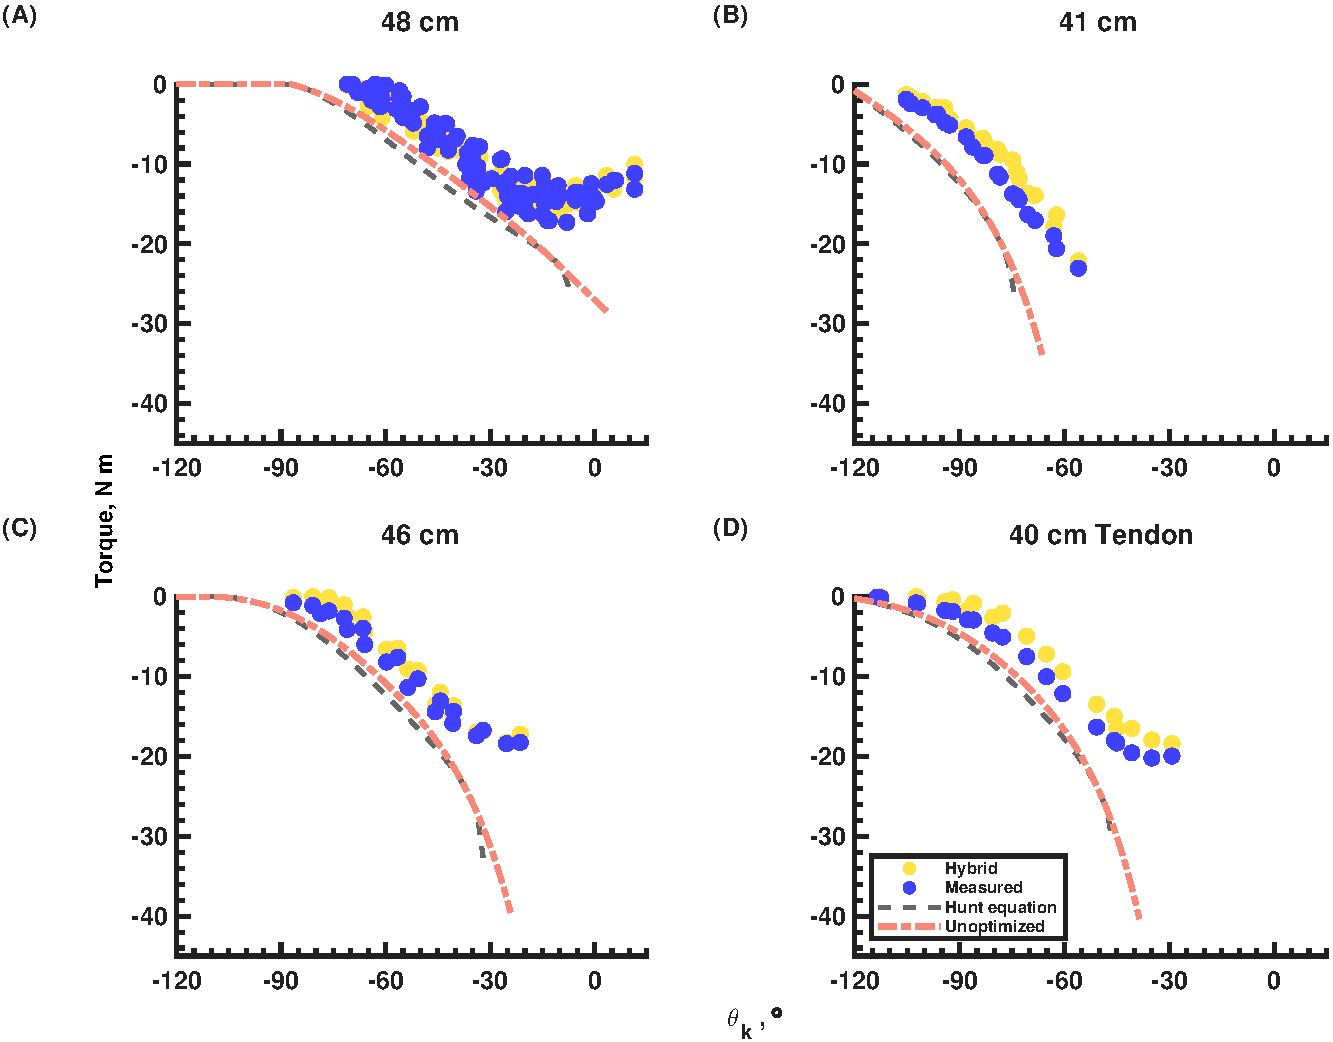
\includegraphics[width=0.9\textwidth]{FlxPin_preopt_publication.pdf}
\end{center}
\caption{Pinned-knee flexor torque before design-parameter optimization: \textbf{(A)} $l_0=\qty{48.5}{\cm}$, \textbf{(B)} $l_0=\qty{41.0}{\cm}$, \textbf{(C)} $l_0=\qty{45.7}{\cm}$, and \textbf{(D)} $l_0=\qty{40.6}{\cm}$ with a \qty{35}{\mm} tendon. Panels \textbf{(A)} and \textbf{(B)} are training tests; \textbf{(C)} and \textbf{(D)} are validation tests. The legend distinguishes measurements, the Hunt model, the improved BPA model, and the hybrid calculation.}\label{fig:FlxPin_preopt}
\end{figure}

\begin{table}[H]
\caption{Lengths $l_0$ (resting BPA) and $l_{\mathrm{ten}}$ (artificial tendon) are both in cm. Pre-optimization pinned-knee flexor torque-prediction goodness of fit per test, comparing the three pre-optimization torque predictions of Figure~\ref{fig:FlxPin_preopt}: the Hunt-equation rigid-body prediction, the unoptimized prediction of the improved BPA characterization, and the back-calculated (hybrid) torque. RMSE and maximum absolute residual (Max.) are in $\mathrm{N\,m}$, and FVU denotes the fraction of variance unexplained.}
\label{tab:FlxPinPreGof}
\begingroup
\renewcommand{\arraystretch}{1}%
\fontsize{10pt}{12pt}\selectfont
\begin{tabular}{@{}cc ccccccccc@{}}
\toprule
& & \multicolumn{3}{c}{\textbf{Hunt equation}} & \multicolumn{3}{c}{\textbf{Improved BPA}} & \multicolumn{3}{c}{\textbf{Back-calculated (hybrid)}} \\
\cmidrule(lr){3-5} \cmidrule(lr){6-8} \cmidrule(l){9-11}
$\boldsymbol{l_{0}}$ (\unit{\cm}) & $\boldsymbol{l_{\text{ten}}}$ (\unit{\cm}) & \textbf{RMSE} & \textbf{FVU} & \textbf{Max.} & \textbf{RMSE} & \textbf{FVU} & \textbf{Max.} & \textbf{RMSE} & \textbf{FVU} & \textbf{Max.} \\
\midrule
48.5 & -- & 5.779 & 1.1761 & 9.798 & 4.871 & 0.8354 & 9.865 & 1.635 & 0.0991 & 3.842 \\
41.0 & -- & 6.633 & 3.2313 & 11.409 & 6.074 & 2.7090 & 9.262 & 2.187 & 0.1184 & 4.243 \\
45.7 & -- & 5.315 & 0.9408 & 9.991 & 4.465 & 0.6640 & 9.536 & 1.246 & 0.0409 & 2.275 \\
40.6 & 3.5 & 3.945 & 0.6750 & 7.527 & 3.226 & 0.4512 & 7.376 & 2.085 & 0.0755 & 3.073 \\
\bottomrule
\end{tabular}
\endgroup
\end{table}



The flexor identification of record is the two-bracket fit of Section~\ref{sec:identification} on the four cross-validation tests; the optimized model follows the measured torque across the range of motion, including the loss of torque near full extension that the rigid-body prediction does not produce (Figure~\ref{fig:FlxPin_optimized}, Tables~\ref{tab:AdoptedXi} and~\ref{tab:FlxPinGof}). The complete five-test comparison before and after correction is provided in Table~\ref{tab:app_gof}.

\begin{figure}[htbp]
\begin{center}
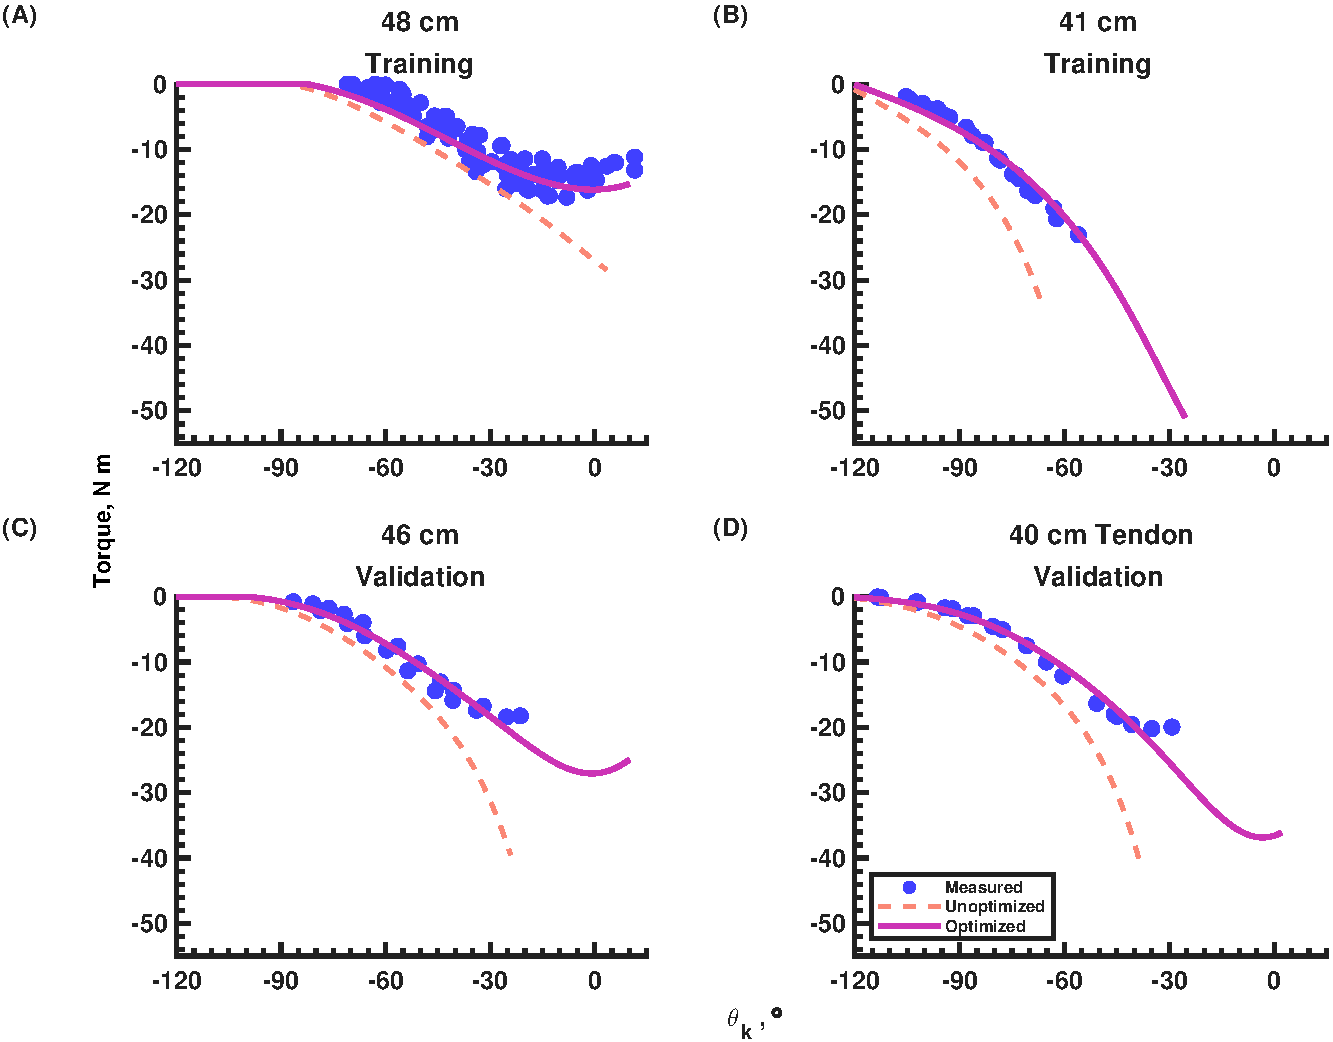
\includegraphics[width=0.9\textwidth]{FlxPin_optimized_publication.pdf}
\end{center}
\caption{Optimized pinned-knee flexor torque: \textbf{(A)} $l_0=\qty{48.5}{\cm}$, \textbf{(B)} $l_0=\qty{41.0}{\cm}$, \textbf{(C)} $l_0=\qty{45.7}{\cm}$, and \textbf{(D)} $l_0=\qty{40.6}{\cm}$ with a \qty{35}{\mm} tendon. Panels \textbf{(A)} and \textbf{(B)} are training tests; \textbf{(C)} and \textbf{(D)} are validation tests. Circles show measurements, dashed curves the improved BPA model, and solid magenta curves the optimized model.}\label{fig:FlxPin_optimized}
\end{figure}

\begin{table}[H]
\caption{Lengths $l_0$ (resting BPA) and $l_{\mathrm{ten}}$ (artificial tendon) are both in cm. Pinned-knee flexor goodness of fit before and after correction, using the identified terms. RMSE and maximum absolute residual (Max.) are in $\mathrm{N\,m}$; FVU is dimensionless.}
\label{tab:FlxPinGof}
\begingroup
\renewcommand{\arraystretch}{1.4}%
\fontsize{10pt}{12pt}\selectfont
\begin{tabular}{@{}cc cccccc@{}}
\toprule
& & \multicolumn{3}{c}{\textbf{Improved BPA}} & \multicolumn{3}{c}{\textbf{Optimized model}} \\
\cmidrule(lr){3-5} \cmidrule(l){6-8}
$\boldsymbol{l_{0}}$ (\unit{\cm}) & $\boldsymbol{l_{\text{ten}}}$ (\unit{\cm}) & \textbf{RMSE} & \textbf{FVU} & \textbf{Max.} & \textbf{RMSE} & \textbf{FVU} & \textbf{Max.} \\
\midrule
\multicolumn{8}{@{}l}{\textbf{Training}} \\
48.5 & -- & 7.617 & 2.1278 & 25.531 & 2.165 & 0.1718 & 5.467 \\
41.0 & -- & 9.694 & 2.1149 & 21.076 & 1.084 & 0.0277 & 1.766 \\
\multicolumn{2}{@{}l}{\hspace*{1em}Mean} & 8.656 & 2.1213 & 23.303 & 1.624 & 0.0998 & 3.617 \\
\midrule
\multicolumn{8}{@{}l}{\textbf{Validation}} \\
45.7 & -- & 8.803 & 1.9380 & 26.264 & 1.368 & 0.0468 & 3.614 \\
40.6 & 3.5 & 6.373 & 0.5935 & 16.859 & 1.611 & 0.0427 & 5.891 \\
\multicolumn{2}{@{}l}{\hspace*{1em}Mean} & 7.588 & 1.2657 & 21.562 & 1.490 & 0.0447 & 4.752 \\
\bottomrule
\end{tabular}
\endgroup
\end{table}

The corrected model reduces mean torque-prediction error in both the training and validation tests, with the optimized curves tracking the measurements across the tested range (Figure~\ref{fig:FlxPin_optimized} and Table~\ref{tab:FlxPinGof}). The baseline uses the same kinematics and force model with the correction terms disabled; Figure~\ref{fig:FlxPin_preopt} separately compares the original rigid-body prediction.



\subsection{Extensor on Pin Joint}

The correction terms reduce mean pinned-knee extensor torque-prediction error in both the training and validation tests (Table~\ref{tab:ExtPinGof}). Figure~\ref{fig:ExtPin_group} compares the measured and predicted torque across knee angle. By inspection, the zero point of the measured torque was shifted to the right of the original model, consistent with an offset opposite in sign to the $\chi_{0}$ term in the previous section. The BPA in Figure~\ref{fig:ExtPin_group}\textbf{(C)} illustrates the pattern: the hybrid-method calculated torque correlates well with the originally predicted torque, while the actual measured torque diverges. The fitted wrapping term $\chi_{3}$ enters the usable-length correction in Equation~\eqref{eq:deltaL}. Table~\ref{tab:ExtPinGof} reports the improvement of the fit. Extensor-specific terms $(\chi_{0}, \chi_{3})$ were specified while stiffness terms $(\chi_{1}, \chi_{2})$ were kept the same as the previous section (see Table~\ref{tab:AdoptedXi}).

\begin{figure}[htbp]
\begin{center}
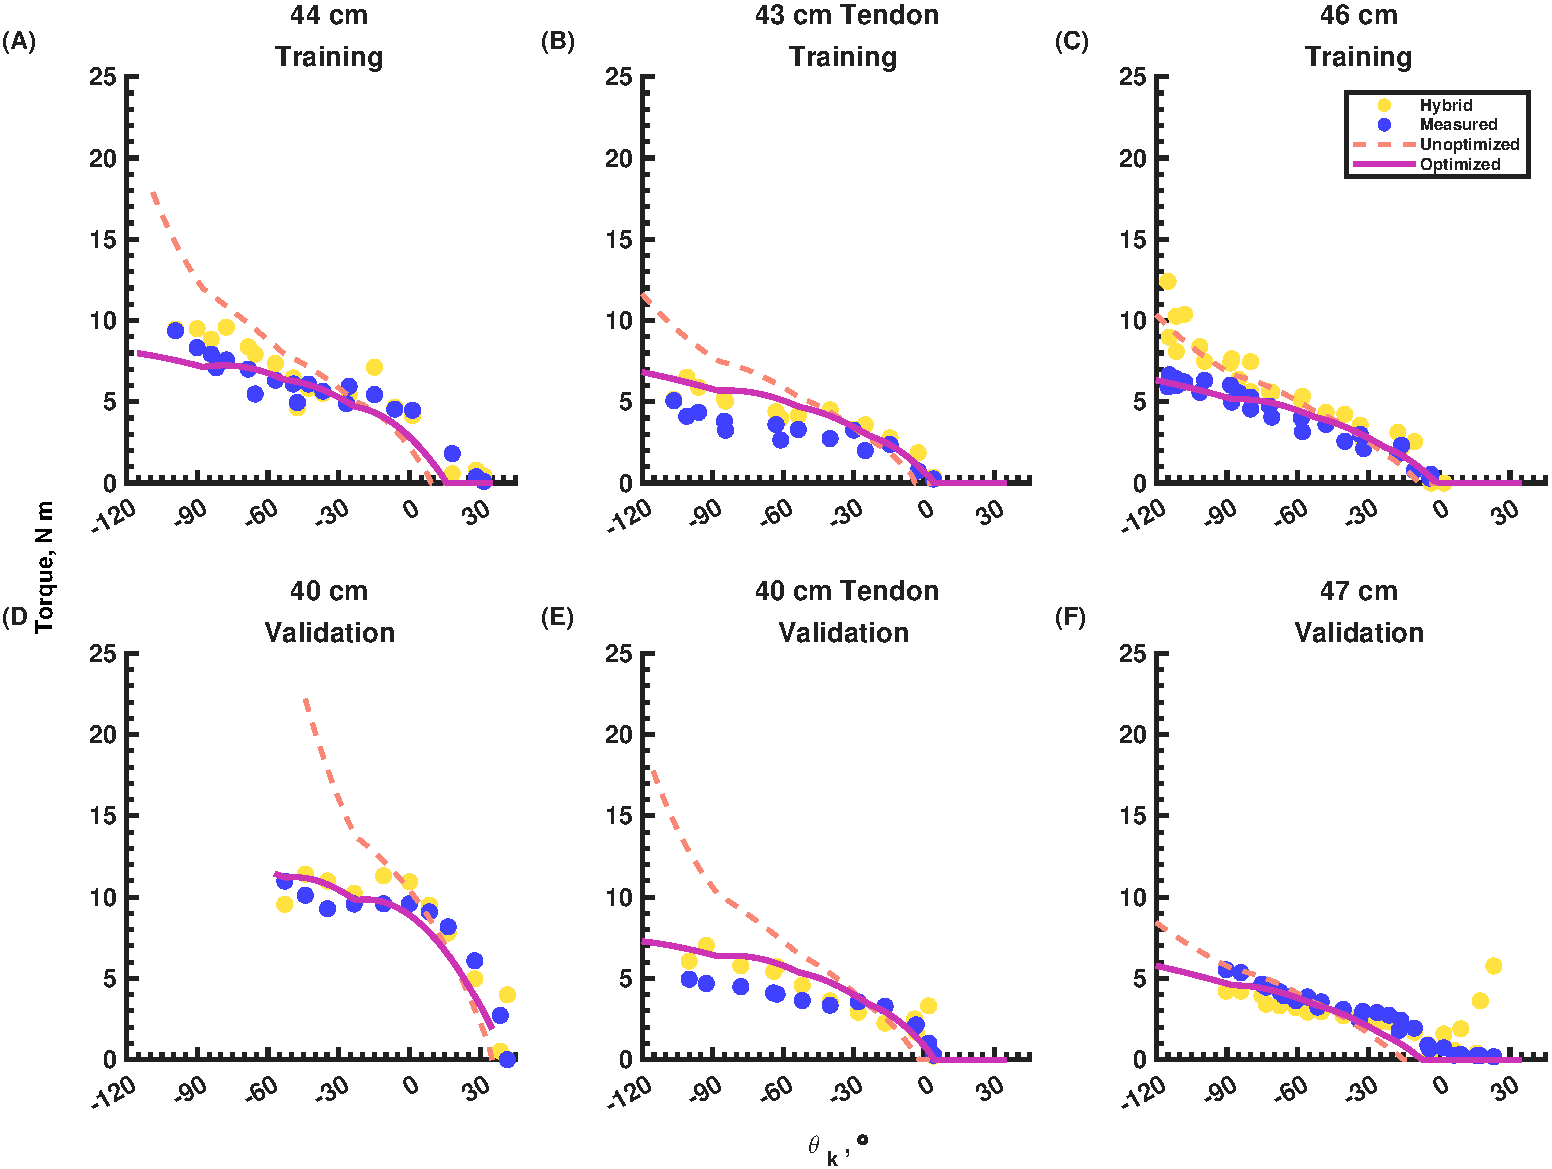
\includegraphics[width=\linewidth,height=0.62\textheight,keepaspectratio]{ExtPin_complete_publication.pdf}
\end{center}
\caption{Optimized pinned-knee extensor torque: \textbf{(A)} $l_0=\qty{43.6}{\cm}$, \textbf{(B)} $l_0=\qty{43.2}{\cm}$ with a \qty{22}{\mm} tendon, \textbf{(C)} $l_0=\qty{45.7}{\cm}$, \textbf{(D)} $l_0=\qty{40.0}{\cm}$, \textbf{(E)} $l_0=\qty{40.0}{\cm}$ with a \qty{40}{\mm} tendon, and \textbf{(F)} $l_0=\qty{46.5}{\cm}$. Panels \textbf{(A)}--\textbf{(C)} are training tests; \textbf{(D)}--\textbf{(F)} are validation tests. The legend applies to all panels.}\label{fig:ExtPin_group}
\end{figure}

\begin{table}[H]
\caption{Pinned-knee extensor goodness of fit before and after correction, with stiffness shared with the flexor. RMSE and maximum absolute residual (Max.) are in $\mathrm{N\,m}$; FVU is dimensionless.}
\label{tab:ExtPinGof}
\begingroup
\renewcommand{\arraystretch}{1}%
\fontsize{10pt}{12pt}\selectfont
\begin{tabular}{@{}cc cccccc@{}}
\toprule
& & \multicolumn{3}{c}{\textbf{Improved BPA}} & \multicolumn{3}{c}{\textbf{Optimized model}} \\
\cmidrule(lr){3-5} \cmidrule(l){6-8}
$\boldsymbol{l_{0}}$ (\unit{\cm}) & $\boldsymbol{l_{\text{ten}}}$ (\unit{\mm}) & \textbf{RMSE} & \textbf{FVU} & \textbf{Max.} & \textbf{RMSE} & \textbf{FVU} & \textbf{Max.} \\
\midrule
\multicolumn{8}{@{}l}{\textbf{Training}} \\
43.6 & -- & 2.437 & 0.9618 & 4.284 & 0.978 & 0.1634 & 1.818 \\
43.2 & 22 & 2.878 & 4.7304 & 4.817 & 1.525 & 1.3270 & 2.481 \\
45.7 & -- & 2.178 & 1.0586 & 4.974 & 0.490 & 0.0535 & 1.206 \\
\multicolumn{2}{@{}l}{\hspace*{1em}Mean} & 2.498 & 2.2503 & 4.692 & 0.997 & 0.5146 & 1.835 \\
\midrule
\multicolumn{8}{@{}l}{\textbf{Validation}} \\
40.0 & -- & 3.092 & 0.5638 & 4.842 & 1.244 & 0.1303 & 2.196 \\
40.0 & 40 & 3.622 & 6.3919 & 7.845 & 1.350 & 0.8878 & 1.890 \\
46.5 & -- & 0.949 & 0.3152 & 2.272 & 0.699 & 0.1714 & 1.559 \\
\multicolumn{2}{@{}l}{\hspace*{1em}Mean} & 2.554 & 2.4236 & 4.986 & 1.098 & 0.3965 & 1.882 \\
\bottomrule
\end{tabular}
\endgroup
\end{table}


\subsection{Extensor on Biomimetic Knee}




I tested the extensor configuration on the biomimetic knee with a $\diameter$\qty{10}{\mm} BPA at $l_{0}=\qty{51.8}{\cm}$. The measured torque fell well below the original prediction (Figure~\ref{fig:Ext10mm_52cm}). Applying the extensor terms identified on the pinned knee improved the prediction: at those terms, the optimized model reached an RMSE of \qty{1.1702}{\newton\meter}, an FVU of 0.6681, and a maximum absolute residual of \qty{2.2088}{\newton\meter}, against \qty{3.0322}{\newton\meter}, 4.4856, and \qty{5.5870}{\newton\meter} for the original rigid-body prediction.

\begin{figure}[htbp]
\centering
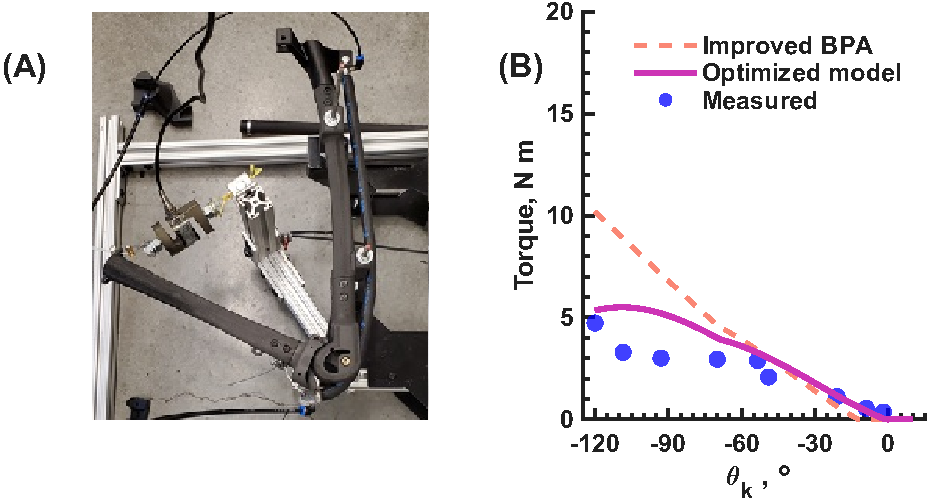
\includegraphics[width=\textwidth]{Ext10mm_52cm_current_publication.pdf}
\caption{Biomimetic-knee extensor test: \textbf{(A)} apparatus with the BPA passing between the femoral condyles; \textbf{(B)} measured torque, the improved BPA baseline, and the optimized model at the identified terms for the \qty{10}{\mm}-diameter, \qty{51.8}{\cm} BPA.}
\label{fig:Ext10mm_52cm}\label{fig:Ext_passthru}
\end{figure}



\subsection{Flexor on Biomimetic Knee}


The shared correction terms reduce torque-prediction error for both biomimetic-knee flexor configurations (Table~\ref{tab:BioTorqueGof}). Figure~\ref{fig:FlxGrp} compares these predictions with the measurements; the bracket frame for the $\diameter$\qty{10}{\mm} BPA is shown in Figure~\ref{fig:bktFrame}\textbf{(C)}, and for the $\diameter$\qty{20}{\mm} BPA in Figure~\ref{fig:bktFrame}\textbf{(D)}. Figure~\ref{fig:FlxGrp}\textbf{(A)} presents the $\diameter$\qty{10}{\mm} actuator at $l_{0}=\qty{41.5}{\cm}$ with a \qty{21}{\mm} artificial tendon ($\diameter$\qty{1.5}{\mm} Shimano bicycle brake cable wrapped four times), pressurized to \qty{604}{\kPa}; the optimized model reached an RMSE of \qty{2.8002}{\newton\meter}, an FVU of 0.8835, and a maximum absolute residual of \qty{4.1201}{\newton\meter}. Figure~\ref{fig:FlxGrp}\textbf{(B)} presents the $\diameter$\qty{20}{\mm} actuator at $l_{0}=\qty{41.5}{\cm}$ with a \qty{14}{\mm} artificial tendon made out of the same brake cable, wrapped three times so that six cable segments share the load, each wrap contributing two tendon lengths and cross-sectional areas. The configuration in Figure~\ref{fig:FlxGrp}\textbf{(B)} was tested at \qty{620}{\kPa}, for which the optimized model reached an RMSE of \qty{2.2070}{\newton\meter}, an FVU of 0.0748, and a maximum absolute residual of \qty{3.7320}{\newton\meter}.

The torque of the single $\diameter$\qty{20}{\mm} flexor actuator shown in Figure~\ref{fig:FlxGrp}\textbf{(B)} did not exceed the magnitude of the maximum human isometric flexion torque between \ang{60} and \ang{100} of knee flexion, and within a $\pm 20\%$ band about the human mean it still fell short of human-level torque between \ang{78} and \ang{103} of flexion. Because operating at \qty{620}{\kPa} across the full desired range of motion would load the printed femur beyond its ultimate strength, single points were also recorded at the reduced pressures \qtylist{560;421;325;281}{\kPa}, which show that the desired range of motion is achievable at reduced pressure. This shortfall in flexion torque defines the target that the attachment-route redesign of Section~\ref{sec:mesh_opt} addresses.

\begin{figure}[p]
\begin{center}
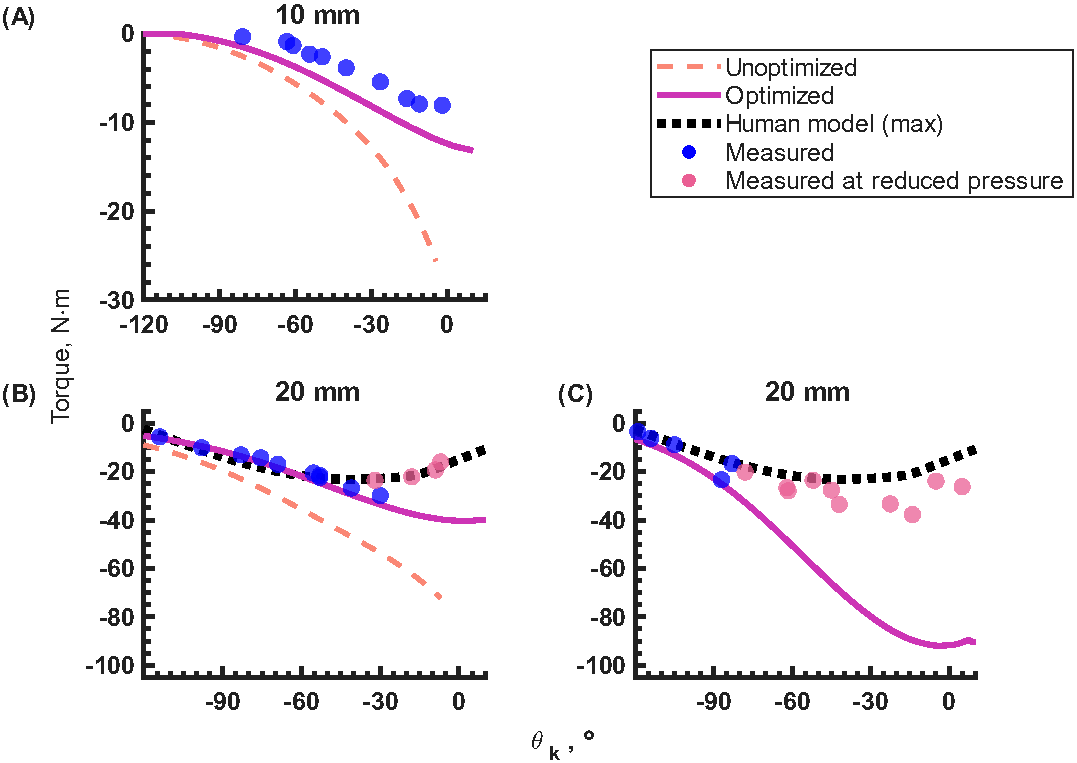
\includegraphics[width=\textwidth,height=0.70\textheight,keepaspectratio]{FlxGrp.pdf}
\end{center}
\caption{Biomimetic-knee flexor torque: \textbf{(A)} a single \qty{10}{\mm} BPA; \textbf{(B)} a single \qty{20}{\mm} BPA. The legend in \textbf{(B)} identifies the measurements, predictions, and human reference.}\label{fig:FlxGrp}
\end{figure}

\begin{table}[htbp]
\centering\small
\caption{Biomimetic-knee goodness of fit before and after design-parameter optimization. RMSE and maximum absolute residual (Max.) are in $\mathrm{N\,m}$; FVU is dimensionless.}
\label{tab:BioTorqueGof}
\begin{tabular}{@{}lrrrrrr@{}}
\toprule
 & \multicolumn{3}{c}{\textbf{Improved BPA}} & \multicolumn{3}{c}{\textbf{Optimized model}} \\
\cmidrule(lr){2-4}\cmidrule(l){5-7}
\textbf{Configuration} & \textbf{RMSE} & \textbf{FVU} & \textbf{Max.} & \textbf{RMSE} & \textbf{FVU} & \textbf{Max.} \\
\midrule
Extensor, $\diameter\qty{10}{\mm}$ & 3.0322 & 4.4856 & 5.5870 & 1.1702 & 0.6681 & 2.2088 \\
Flexor, $\diameter\qty{10}{\mm}$ & 7.4513 & 5.5612 & 13.3163 & 2.8002 & 0.8835 & 4.1201 \\
Flexor, $\diameter\qty{20}{\mm}$ & 14.8064 & 3.3672 & 23.7218 & 2.2070 & 0.0748 & 3.7320 \\
\bottomrule
\end{tabular}
\end{table}




\section{Discussion}

\subsection{Reasons for the Correction Terms}\label{sec:disc_error}

The correction terms of Section~\ref{sec:improved_model} exist because the physical transmission between the actuator and the joint is neither rigid nor lossless, and each term names one family of physical reasons. A constant length offset $\chi_{0}$ exists because of manufacturing and positioning tolerances: the printed bone segments, the machined knee links, and the end-cap fittings each carry dimensional tolerance, and the accumulated discrepancy appears as a length that is consistently shorter than the predicted path at every joint angle, including at zero load where no compliance can act. The stiffness terms $\chi_{1}$ and $\chi_{2}$ exist because loaded components displace: the isometric system is not rigid, and there is compliance in the winch cable of the test stand, the artificial tendons, and the cantilevered attachment brackets. The wrapping-loss term $\chi_{3}$ exists because a BPA that bends over the joint loses usable contraction length that no straight-line model accounts for; at high flexion the same loading was observed to stretch and compress shorter-$l_{0}$ actuators and to slip the BPA off the anterior head of the femur bolt by up to \qty{\pm 20}{\mm}, changing both the force vector and the torque.

Wrapping a BPA around the knee remains an approximation with inherent error (Figure~\ref{fig:Ext_passthru}): high actuator force and a short moment arm make the torque sensitive to attachment deflection and small geometric errors \citep{young_analyzing_2019}. The pinned-knee tests therefore separate actuator-force error from attachment-compliance and routed-geometry error, and applying the identified terms to the biomimetic knee tests them where the moment arm and the instantaneous center of rotation move with knee angle. Isometric testing establishes a static capacity envelope; velocity dependence, damping, and behavior under controlled speed and load remain unidentified.

\subsection{Design-Factor Optimization}\label{sec:ongoing}

The results figures use the two-stage identification of Section~\ref{sec:identification}. Relative to the zero-correction baseline, the optimized model reduces mean RMSE by 81\,\% on the flexor training tests and 80\,\% on the flexor validation tests (Table~\ref{tab:FlxPinGof}), and by 60\,\% on the extensor training tests and 57\,\% on the extensor validation tests (Table~\ref{tab:ExtPinGof}); on the biomimetic extensor it reduces FVU by 85\,\% (Table~\ref{tab:BioTorqueGof}). Table~\ref{tab:AdoptedXi} records the identified terms: the stiffness pair is shared, and the wrapping factor was identified on the extensor and applied to wrapping in the redesigned flexor. The genetic multiobjective solver is retained for the identification, where the Pareto front is required for holdout validation, and the surrogate-plus-pattern-search pipeline serves the route redesign (Section~\ref{sec:mesh_opt}); the search bounds are recorded in Appendix~\ref{app:model_geometry} (Table~\ref{tab:app_opt_bounds}).

\begin{table}[htbp]
\centering\small
\caption{Adopted correction terms. The effective stiffness pair is shared; $\chi_3$ was identified on the extensor and is applied to wrapping in the redesigned flexor.}
\label{tab:AdoptedXi}
\begin{tabular}{@{}lrrrr@{}}
\toprule
Configuration & $\chi_{0}$ (m) & $\chi_{1}$ (N/m) & $\chi_{2}$ (N/m) & $\chi_{3}$\\
\midrule
Flexor & $0.00394$ & $3.998\times10^{4}$ & $1.473\times10^{4}$ & --\\
Extensor & $-0.00638$ & $3.998\times10^{4}$ & $1.473\times10^{4}$ & $0.158$\\
\bottomrule
\end{tabular}
\end{table}

The original placement methods selected routes by predicted torque under rigid-attachment assumptions; the isometric tests show those predictions require the compliance corrections before they can guide hardware selection, so the redesigned routes evaluate every candidate through the corrected force balance. On the biomimetic knee the shared terms transfer at an FVU of 0.8835 for the \qty{10}{\mm} flexor and 0.0748 for the \qty{20}{\mm} flexor (Table~\ref{tab:BioTorqueGof}); the larger error for the smaller actuator limits transfer across configurations, and the redesigned two-BPA routes provide the further physical test of Section~\ref{sec:redesign_physical}.

\subsection{Redesigned Routes for the Biomimetic Robot Model}\label{sec:route_redesign_results}

The redesigned routes combine the existing biomimetic robot geometry with human-muscle torque references. The surrogate-plus-pattern-search procedure of Section~\ref{sec:constrained_redesign} uses the correction terms in Table~\ref{tab:AdoptedXi}, two \qty{20}{\mm} BPAs per route, a \qty{620}{\kPa} pressure ceiling, and a maximum usable contraction of 0.255. Both direct routes meet the required torque envelope (Table~\ref{tab:redesigned_route_capacity}).

\begin{table}[htbp]
\centering
\caption{Predicted direct-route torque capacity on the biomimetic robot model. Both margin rows use the selected human-muscle torque magnitude as their denominator.}
\label{tab:redesigned_route_capacity}
\small
\begin{tabularx}{\textwidth}{@{}lXX@{}}
\toprule
 & \textbf{Extensor} & \textbf{Flexor}\\
\midrule
Predicted torque (N\,m) & 35.45 to 109.4 & $-81.23$ to $-3.864$\\
Human reference torque (N\,m) & 20.25 to 50.32 & $-23.16$ to $-2.461$\\
Minimum predicted margin & $5.02\,\%$ & $5.01\,\%$\\
Required design allowance & $5\,\%$ & $5\,\%$\\
Angle of minimum margin & \ang{-20.2} & \ang{-106.9}\\
\bottomrule
\end{tabularx}
\end{table}

The cam-assisted extensor allows the tibial route points to trace a profile rather than remain fixed (Figure~\ref{fig:ExtensorRoute_redesigned}). Table~\ref{tab:cam_route_summary} summarizes the resulting capacity and geometry. The flexor uses two separately evaluated BPA paths and the wrapping factor identified on the extensor. Each route family minimizes its own weighted penalty sum; objective values are not directly comparable. These are mechanical design predictions; incorporation into the converted neuromechanical models remains future work.

The cam summaries use two different normalizations. For the evaluated knee-angle grid $\Theta$, let $M_h(\theta)$ be the human-reference torque, $M_{h,\max}$ its peak magnitude, and $M_{\mathbf{k}}(\theta)$ the predicted knee-axis torque. The minimum surplus above the required envelope and the minimum relative margin above the human reference are
\begin{equation}
\begin{aligned}
s_{\mathrm{req}} &= \min_{\theta\in\Theta}\frac{\lvert M_{\mathbf{k}}(\theta)\rvert-1.05\lvert M_h(\theta)\rvert}{M_{h,\max}},\\
m_h &= \min_{\theta\in\Theta}\frac{\lvert M_{\mathbf{k}}(\theta)\rvert-\lvert M_h(\theta)\rvert}{\lvert M_h(\theta)\rvert}.
\end{aligned}
\label{eq:cam_summary_definitions}
\end{equation}

\begin{figure}[p]
\centering
\begin{minipage}[t]{0.32\textwidth}\vspace{0pt}\centering
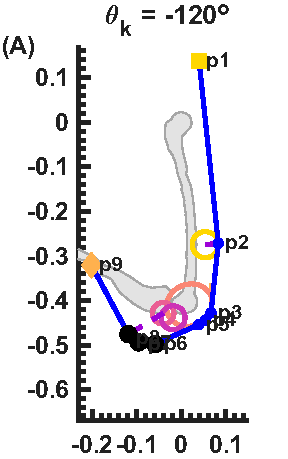
\includegraphics[width=\linewidth]{cam_pose_A.pdf}
\end{minipage}\hfill
\begin{minipage}[t]{0.32\textwidth}\vspace{0pt}\centering
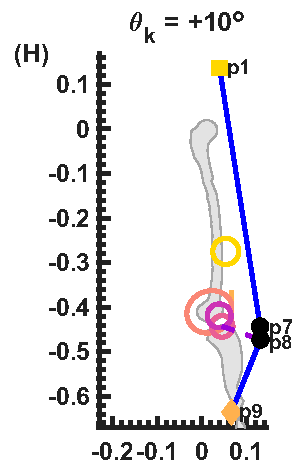
\includegraphics[width=\linewidth]{cam_pose_H.pdf}
\end{minipage}\hfill
\begin{minipage}[t]{0.32\textwidth}\vspace{0pt}\centering
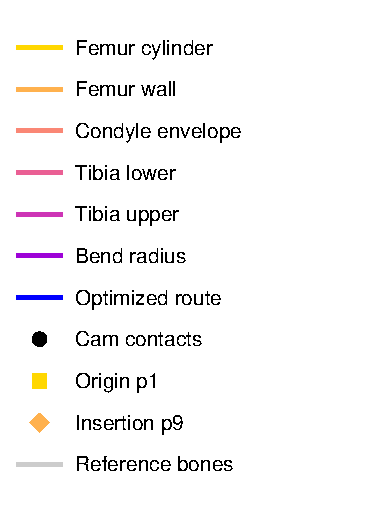
\includegraphics[width=\linewidth]{cam_current_legend.pdf}
\end{minipage}
\par\medskip
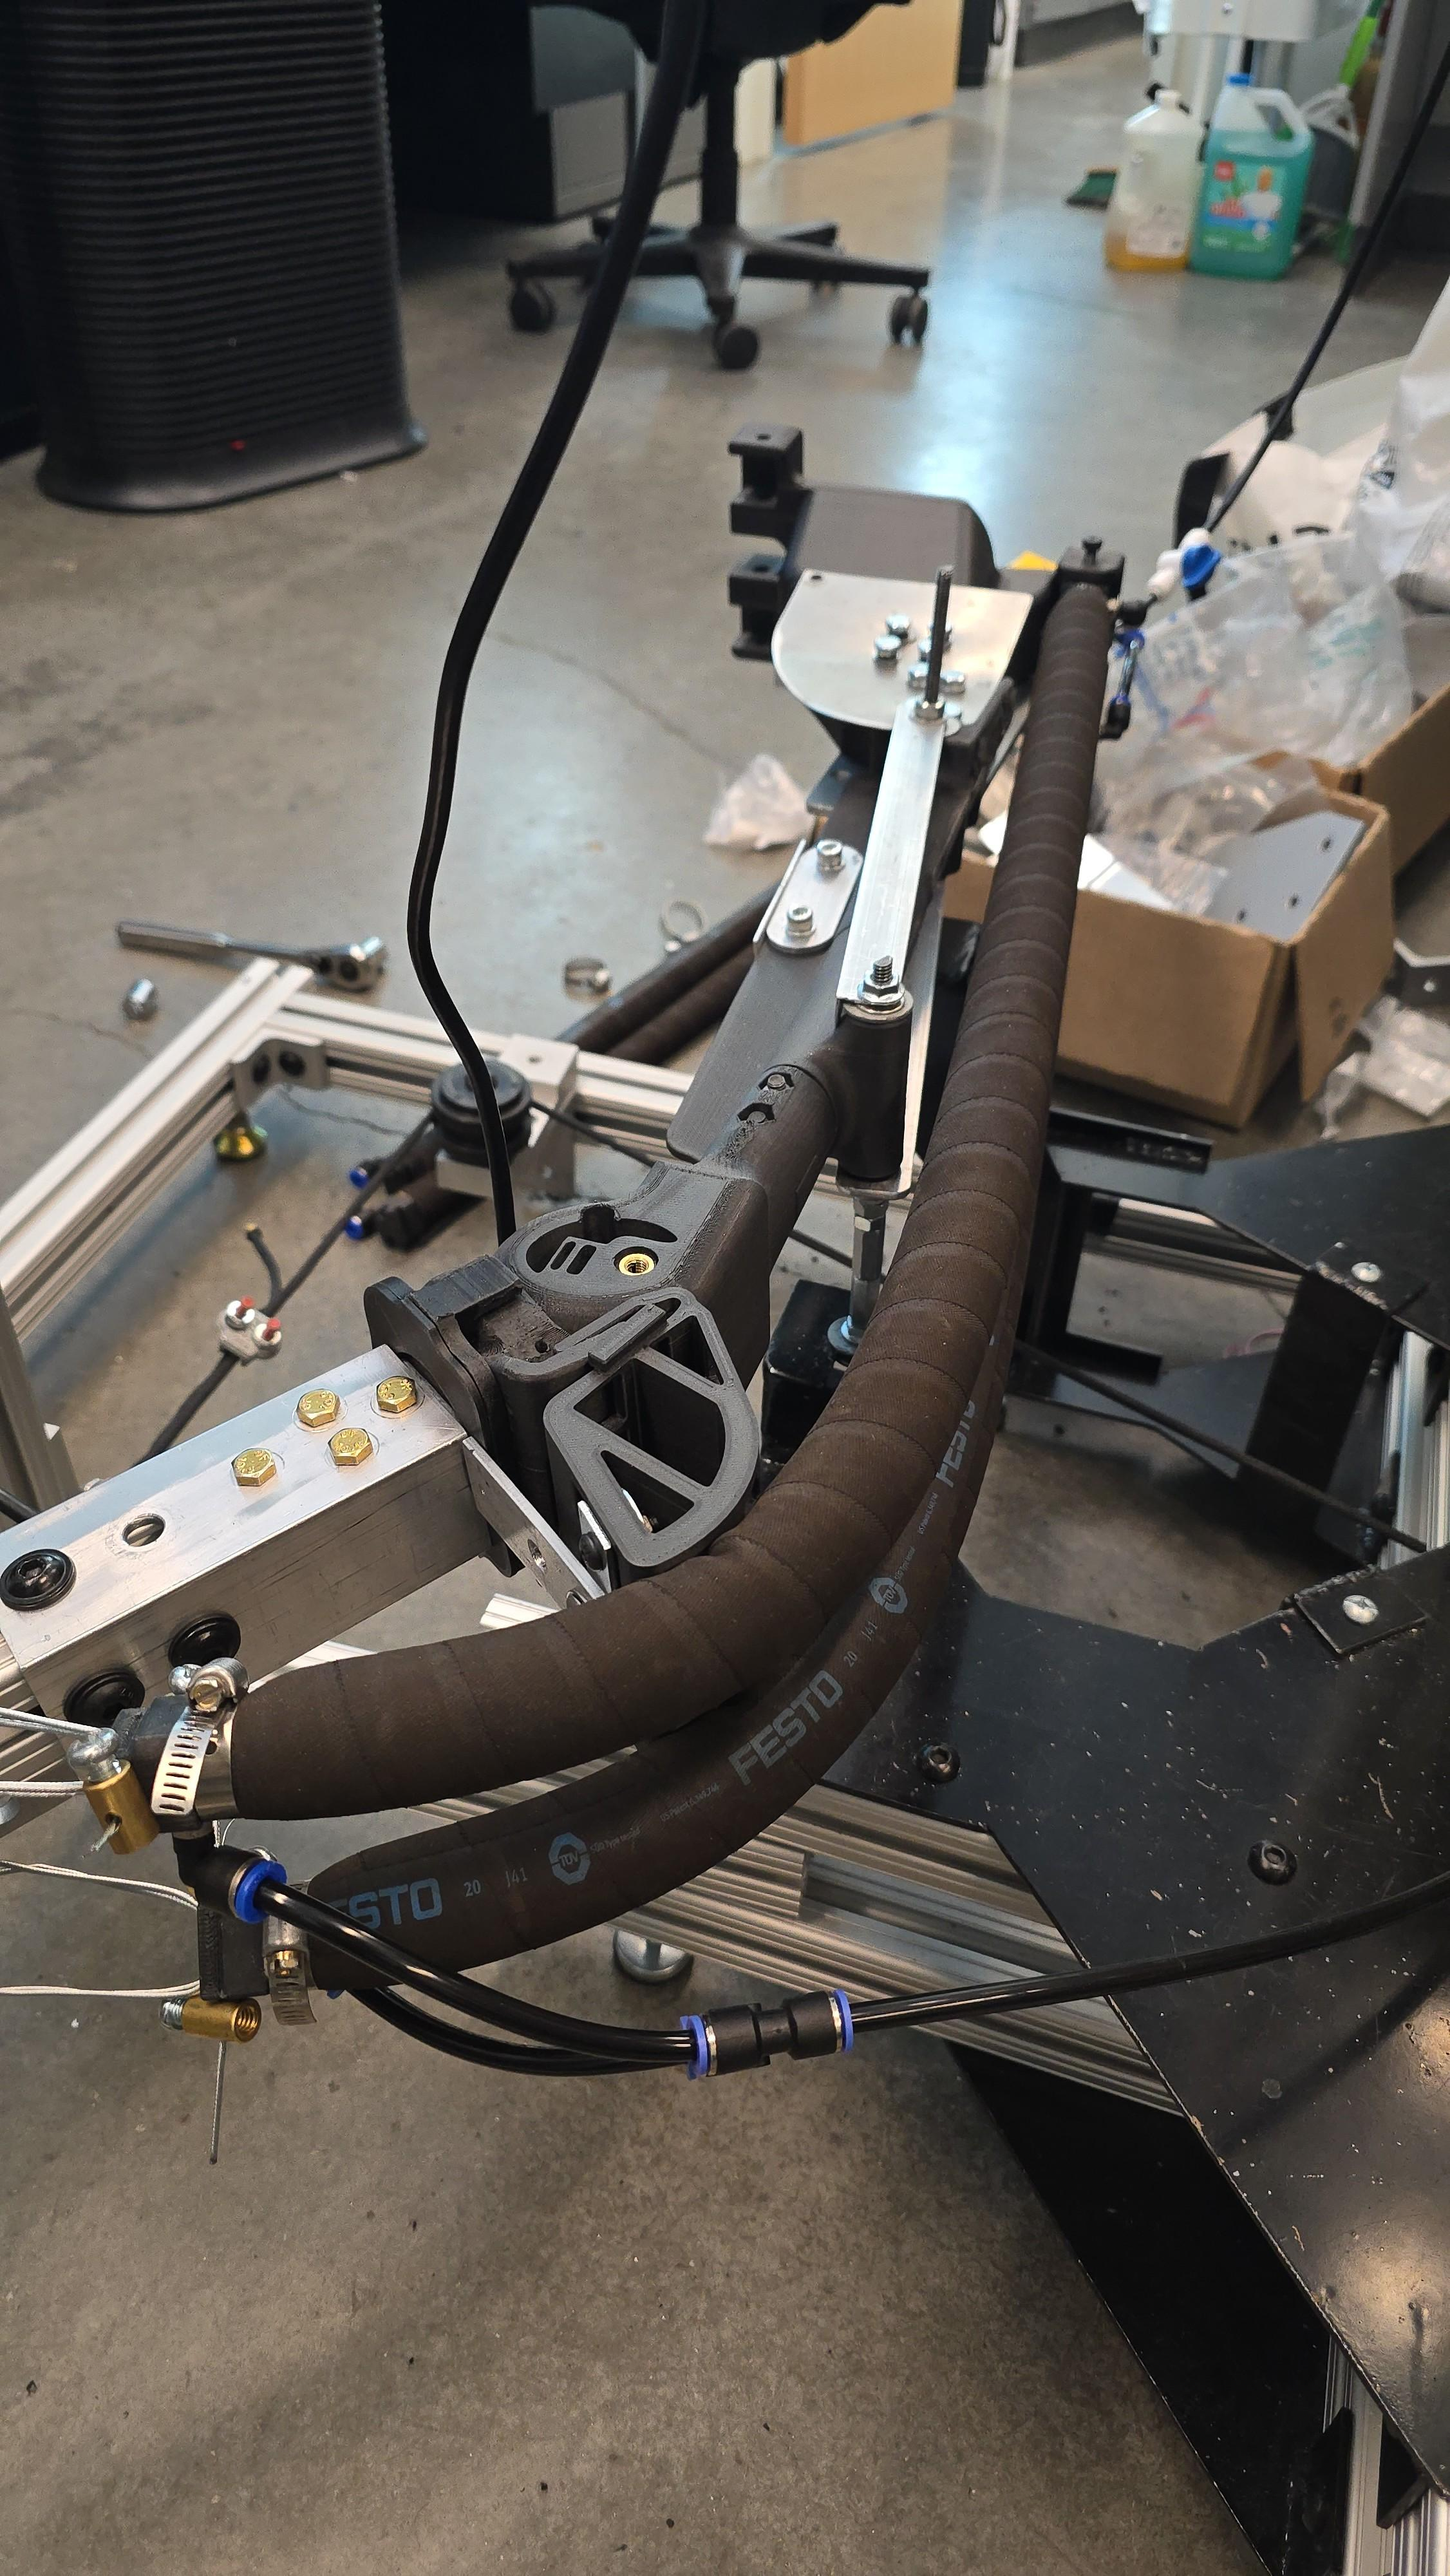
\includegraphics[width=0.46\textwidth,height=0.31\textheight,keepaspectratio]{cam_extensor_hardware.jpg}
\caption{Cam-extensor geometry at \ang{-120} (A) and \ang{10} (H), with the assembled two-BPA hardware below. Panel letters match the complete sequence in Figures~\ref{fig:app_cam_AF} and~\ref{fig:app_cam_GH}.}
\label{fig:ExtensorRoute_redesigned}
\end{figure}


\begin{table}[htbp]
\centering
\caption{Predicted cam-extensor capacity and routing geometry for the biomimetic robot model. The torque summaries are defined in Equation~\eqref{eq:cam_summary_definitions}.}
\label{tab:cam_route_summary}
\begin{tabular}{@{}lr@{}}
\toprule
\textbf{Quantity} & \textbf{Value}\\
\midrule
Minimum surplus / peak human torque, $s_{\mathrm{req}}$ & $+30.83\,\%$\\
Minimum pointwise margin above human, $m_h$ & $+39.77\,\%$\\
Pressure to meet required envelope & \qtyrange{269}{507}{\kPa}\\
Pressure floor used in model & \qty{150}{\kPa}\\
Tibial bend radius & \qty{96.9}{\mm}\\
Femoral-condyle clearance at \ang{10} & \qty{43.1}{\mm}\\
Moment-arm range & \qtyrange{59.4}{102.8}{\mm}\\
Mean moment arm & \qty{72.4}{\mm}\\
\bottomrule
\end{tabular}
\end{table}

Pressure headroom permits the required torque below the supply ceiling. In my operating experience, the present manifold has an approximately~\qty{200}{\kPa} lower operating limit, which can restrict minimum controllable nonzero torque magnitude while the BPAs are taut. The saved design calculation used a~\qty{150}{\kPa} pressure floor.

\subsection{Exceeding Human Torque Magnitude}\label{sec:redesign_physical}

Both redesigned routes met or exceeded their selected human-muscle reference torques at the measured knee angles. The cam-assisted extensor was tested at nine isometric configurations and the two-BPA flexor at fifteen, spanning \ang{-119} to \ang{5}. The analysis transforms the measured load-cell wrench to the moving knee center and evaluates the model at each measured angle and pressure. Table~\ref{tab:final_test_dimensions} in Appendix~\ref{app:model_geometry} records the measured per-actuator dimensions and distinguishes them from the shared prediction inputs. Figures~\ref{fig:extensor_physical_final} and~\ref{fig:flexor_physical_final} compare these results with the selected human-muscle targets and the optimized \qty{620}{\kPa} predictions.

The extensor measurements meet or exceed the vastus medialis reference torque at the measured angles. Measured extension torque ranges from \qty{29.02}{\newton\meter} to \qty{51.17}{\newton\meter}, with margins of \qtyrange{0.24}{3.52}{\newton\meter}, at pressures of \qtyrange{256}{488}{\kPa}. The measured torque exceeds the pressure-specific prediction at eight angles, by up to \qty{13.75}{\newton\meter}; at \ang{-86.5}, the measurement exceeds the human reference and is \qty{2.06}{\newton\meter} below the pressure-specific prediction. This prediction uses the recorded angle and pressure with the modeled route. It is not the hybrid calculation, which additionally requires measured muscle length and moment arm.

The flexor measurements meet or exceed the biceps femoris short-head reference magnitude, with margins from \qty{0.42}{\newton\meter} at \ang{-105} to \qty{17.0}{\newton\meter} at \ang{-14}. Agreement with the pressure-specific prediction remains uneven. These measurements support torque capacity at the sampled configurations; variable test pressure and discrete sampling do not establish a measured full-pressure envelope between every pair of angles.

\begin{figure}[p]
\centering
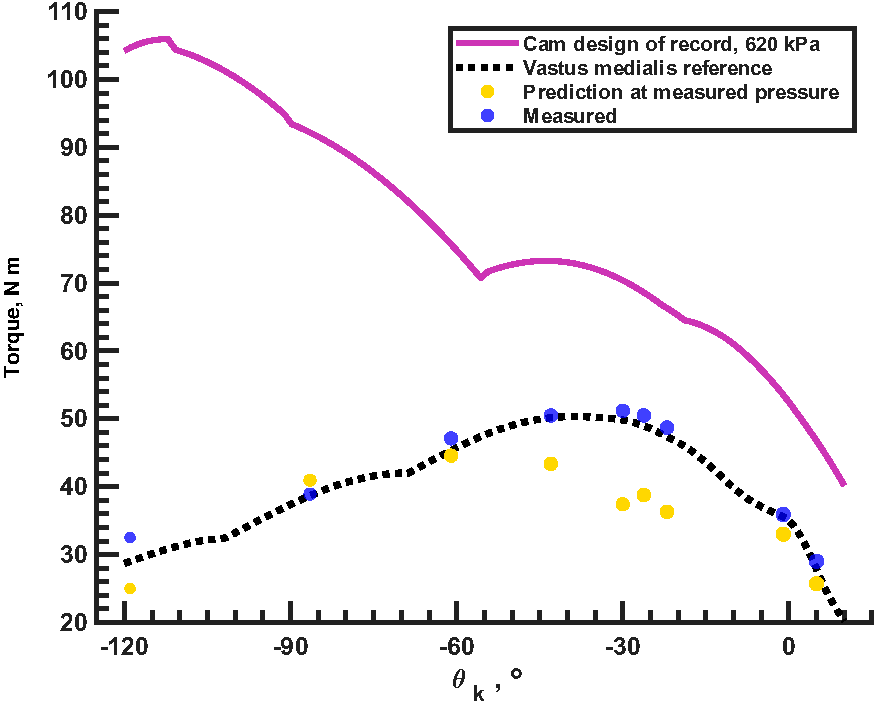
\includegraphics[width=0.97\textwidth]{Ext20mm_physical_20261026_publication.pdf}
\caption{Cam-extensor measurements, pressure-specific predictions, the optimized \qty{620}{\kPa} curve, and the vastus medialis reference. Marker area scales with pressure. Series follow the plot legend.}
\label{fig:extensor_physical_final}
\end{figure}

\begin{figure}[p]
\centering
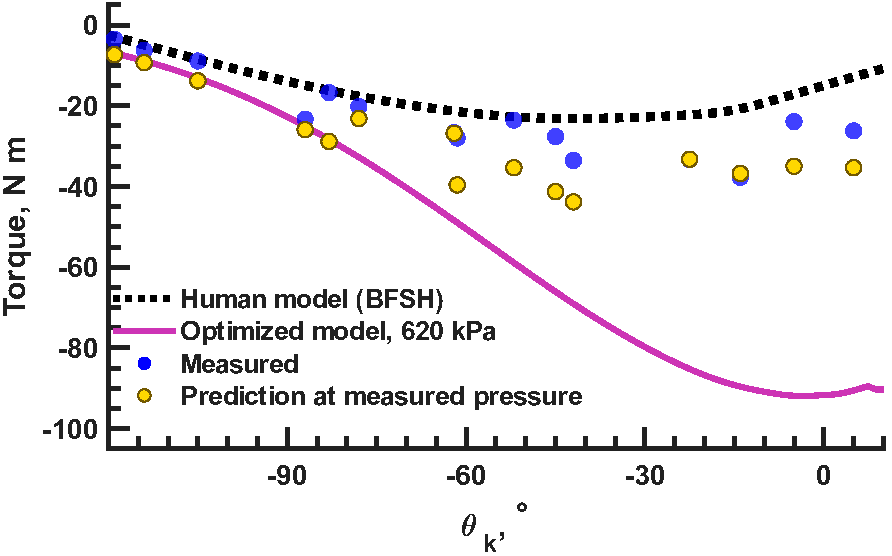
\includegraphics[width=0.97\textwidth]{Redesigned_flexor_pressure_publication.pdf}
\caption[Physical tests of the redesigned flexor route]{Two-BPA flexor tests (nominal \qty{562}{\mm} plot label); the installed resting lengths were \qtylist{561;560}{\mm}. Blue points are measured torques; gold points are model predictions at the measured angles and pressures. The solid magenta curve is the optimized \qty{620}{\kPa} prediction, and the black dotted curve is the human biceps femoris short-head target.}
\label{fig:flexor_physical_final}
\end{figure}

\subsection{Mono- and Bi-Pulley Tendon Routing}\label{sec:disc_pulley}

Reeving the artificial tendon through a reverse block-and-tackle trades transmitted force for tendon travel (Figure~\ref{fig:reverse_pulley_principle}). Let $F_{\mathrm{BPA}}$ be the total input force, $n$ the number of cable parts supporting the moving block, $\Delta\ell_{\mathrm{BPA}}$ the BPA contraction, and $\Delta s_t$ the tendon travel. For an ideal massless cable and frictionless pulleys,
\begin{equation}
F_t=\frac{F_{\mathrm{BPA}}}{n},\qquad
\Delta s_t=n\Delta\ell_{\mathrm{BPA}}.
\label{eq:reverse_pulley_ideal}
\end{equation}
The illustrated two-BPA input is $F_{\mathrm{BPA}}=2F_{20}$; with $n=2$, $F_t=F_{20}$ and tendon travel doubles. The BPA-origin reaction magnitude is $F_{R,\mathrm{origin}}=F_{\mathrm{BPA}}$. Reeving, rather than the number of pulley wheels alone, determines $n$; the travel multiplier used in the route calculations is $G=n$.

This trade can extend the RoM over which a route meets its torque requirement. At $G=n=1$, force and travel ratios relative to the combined BPA input are unity, recovering direct transmission. The design calculations retain internal-load and mount-deflection effects in their stiffness-aware force balance. Appendix~\ref{sec:app_routing_extensions} gives the specific optimized knee-route comparisons and the five-site transmission study (Figures~\ref{fig:PulleySurfaces} and~\ref{fig:PulleyMargins_resolved}); its biarticular evaluation planes hold the adjacent joint fixed, and physical verification remains future work.

\begin{figure}[htbp]
\centering
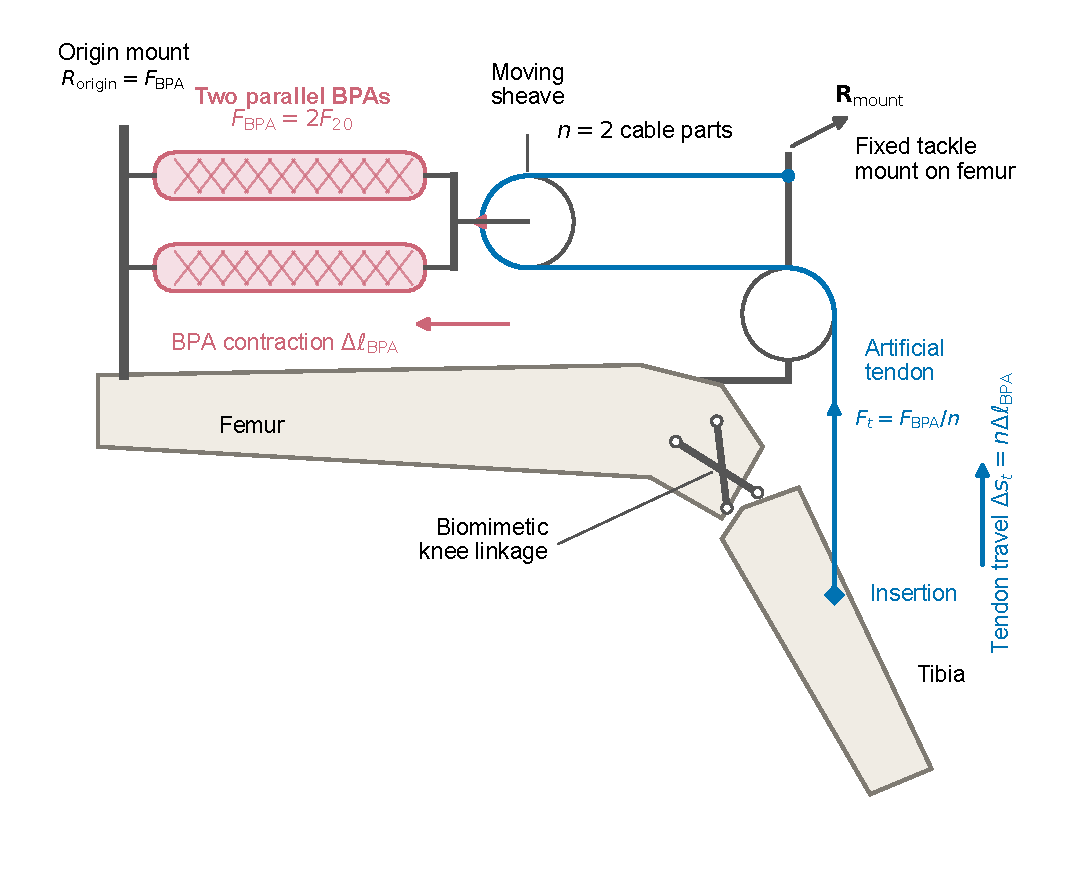
\includegraphics[width=0.96\textwidth,height=0.62\textheight,keepaspectratio]{reverse_pulley_biomimetic.pdf}
\caption[Two-BPA reverse-pulley actuation of a biomimetic knee]{Example of two parallel BPAs actuating a biomimetic knee through a two-part reverse tackle.}
\label{fig:reverse_pulley_principle}
\end{figure}

\subsection{Whole-Leg Transmission Capability}

As a proof of concept for the whole tool chain, I applied the transmission search to the robot-leg muscle routing of my master's model \citep{bolen_determination_2019}: the expanded design selects the best transmission configuration at each of the 27 actuator sites (Table~\ref{tab:survey_dofs_sizes}) and re-solves actuator and tendon lengths on the inherited routing.\label{sec:masters_updated} Each site is evaluated against its same-named Gait2392 muscle \citep{delp_opensim_2007,seth_opensim_2018} on a $5\times5$ grid sampling combinations of two joint coordinates at \qty{620}{\kPa} \citep{bolen_2026}: a cell meets the requirement when the taut BPA's torque has the human torque's sign and at least its magnitude, and the reported coverage is the unweighted mean over sites. The baseline substitutes four parallel \qty{20}{\mm} BPAs at the eight nominal \qty{40}{\mm} sites. Under matched ideal pressure, braid geometry, and contraction, maximum force scales with diameter squared, giving this parallel group the same theoretical maximum force as one \qty{40}{\mm} BPA. The comparison combines transmission, actuator sizing, and the diameter substitution; it does not isolate any one contribution.

Mean human-torque coverage improves from \qty{37.28}{\percent} to \qty{65.19}{\percent}, improving at 23 sites and tying at four, while mean active-force coverage (positive insertion tension, regardless of torque) rises from \qty{92.44}{\percent} to \qty{98.81}{\percent}; positive tension alone does not meet the torque requirement. Table~\ref{tab:CapabilitySurvey} summarizes the means, and Table~\ref{tab:capability_by_site} gives the per-site coverage.

\begin{table}[htbp]
\centering
\caption{Mean torque and active-force coverage across 27 actuator sites at \qty{620}{\kPa}.}
\label{tab:CapabilitySurvey}
\begin{tabular}{@{}lcc@{}}
\toprule
\textbf{Configuration} & \textbf{Human torque met (\%)} & \textbf{Active force (\%)} \\
\midrule
Baseline & 37.28 & 92.44 \\
Transmission configurations & 65.19 & 98.81 \\
\bottomrule
\end{tabular}
\end{table}

With the actuator side of the leg corrected, physically validated, and redesigned to meet human-scale torque, the dissertation turns to the sensory side: Chapter~\ref{ch:database} assembles the measured afferent responses that the synthetic nervous system of Chapter~\ref{ch:sns} draws on.
